\documentclass[a4paper]{article}

\usepackage[utf8]{inputenc}
\usepackage[T1]{fontenc}
\usepackage[italian]{babel}

\usepackage[margin=4.2cm, top=1.5cm, bottom=2.5cm]{geometry}

\usepackage{siunitx}
\usepackage{amsmath}
\usepackage{amssymb}
\usepackage[hidelinks]{hyperref}
\usepackage{graphicx}
\usepackage[font={sf}]{caption}
\usepackage{subcaption}
\usepackage{pdflscape}
\usepackage{makecell}

\setlength{\marginparwidth}{95pt}
\let\oldmarginpar\marginpar
\renewcommand\marginpar[1]{\oldmarginpar{\scriptsize\sffamily #1}}

\sisetup{%
separate-uncertainty=true,
multi-part-units=single,
exponent-product=\cdot}

\frenchspacing

\title{Relazione di laboratorio:\\
Esperienza 1. Flusso di raggi cosmici (base)}
\author{Andrea Marasciulli
\and Giacomo Petrillo
\and Roberto Ribatti}
\date{20 novembre -- 15 dicembre 2017}

\begin{document}

\maketitle

\begin{abstract}
	Usando lastre di scintillatore plastico rileviamo il flusso di raggi cosmici.
	Avvalendoci di un piccolo scintillatore mobile montato su una ghiera basculante,
	misuriamo con una precisione dinamica di \SI{\pm 5}{cm} la traiettoria delle faine nel sottotetto.
\end{abstract}

\tableofcontents

\section{Introduzione}

\subsection{Obiettivo}

Vogliamo misurare il tasso per unità di superficie orizzontale
dei raggi cosmici che passano nel laboratorio.
Vedremo che possiamo misurare solo il tasso di muoni.

\subsection{Apparato}

\begin{figure}
	\center
	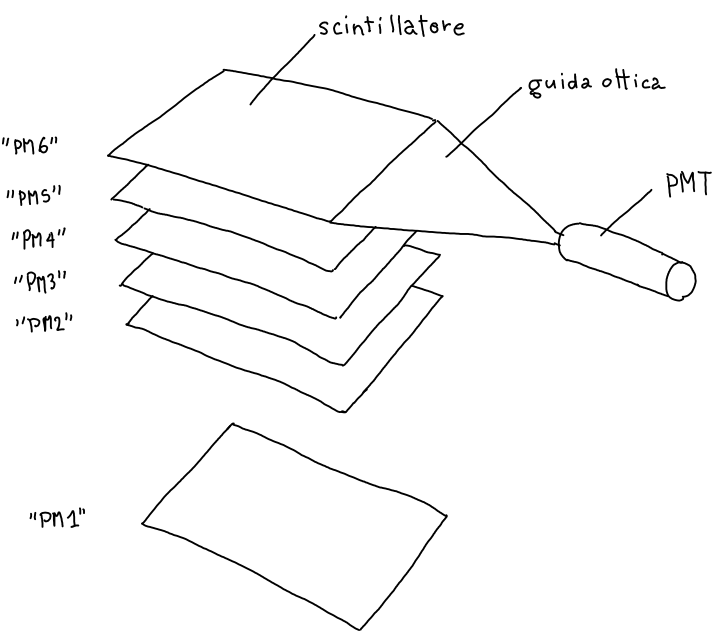
\includegraphics[width=\textwidth]{apparato}
	\caption{\label{fig:apparato}
	Apparato di misura.
	La struttura portante non è disegnata.
	La guida ottica e il tubo fotomoltiplicatore (PMT) sono disegnati solo per il PM6.}
\end{figure}

Abbiamo a disposizione 6 lastre di scintillatore plastico
posizionate orizzontali e allineate verticalmente,
che non possiamo spostare,
collegate a tubi fotomoltiplicatori (vedi \autoref{fig:apparato}).


\section{Teoria}

\subsection{Raggi cosmici al livello del suolo}  % titolo provvisorio

I raggi cosmici primari sono particelle accelerate da sorgenti astrofisiche che colpiscono continuamente l'atmosfera terrestre. Interagendo con i nuclei in alta atmosfera producono flussi di particelle secondarie che a loro volta interagiscono o decadono provocando sciami di particelle.

Al livello del suolo i raggi cosmici carichi sono costituiti principalmente da muoni
e in minor parte da elettroni (e positroni),
come mostrato in Figura~\ref{fig:vertical_angular}\subref{fig:vertical_flux},
dove è riportato il flusso verticale integrato ad una latitudine geomagnetica di $\sim \SI{40}{\degree}$ in funzione della loro energia cinetica. Dal grafico è anche possibile notare come i muoni in arrivo abbiano in pratica tutti energia $>\SI{500}{\MeV}$ e siano perciò considerabili MIP.

\begin{figure}
	\begin{subfigure}[t]{0.48\textwidth}
		\centering
		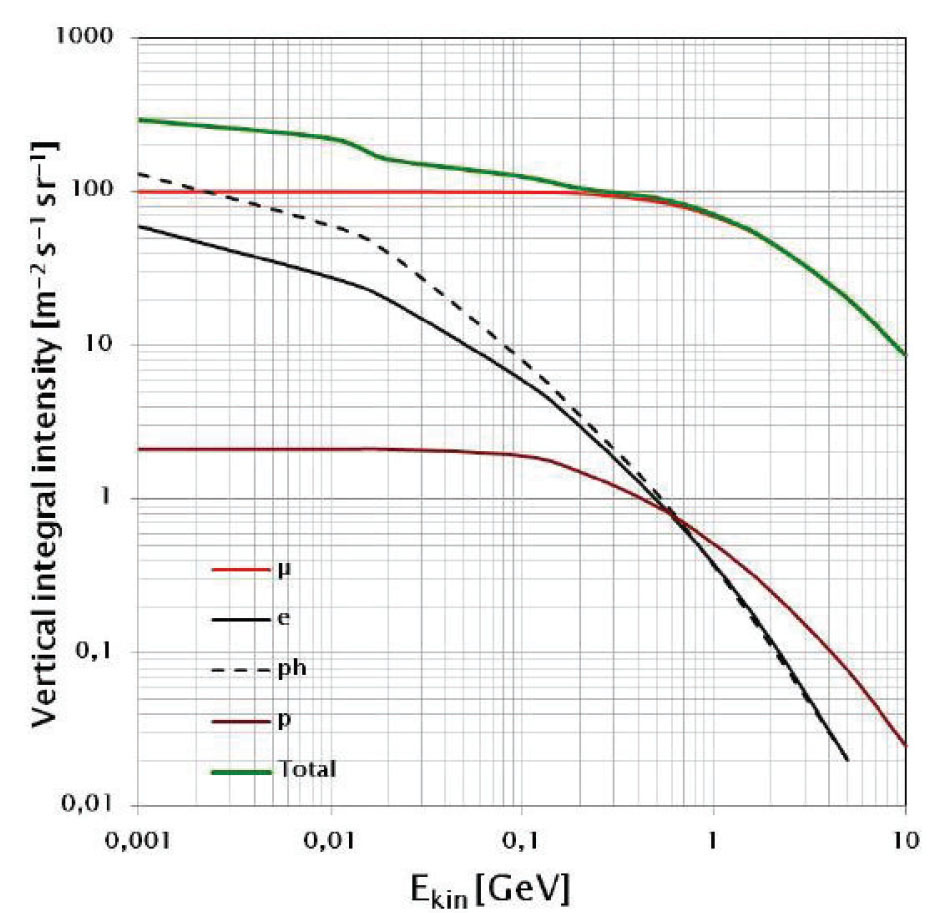
\includegraphics[width=\textwidth]{vertical_flux}
		\caption{\label{fig:vertical_flux}
		Flusso verticale integrato dei raggi cosmici (per ciascuna componente)
		mediato su un ciclo solare di 11 anni al livello del mare
		ad una latitudine geomagnetica di $\sim \SI{40}{\degree}$ in funzione dell'energia cinetica.}
	\end{subfigure}
	\hfill
	\begin{subfigure}[t]{0.48\textwidth}
		\centering
		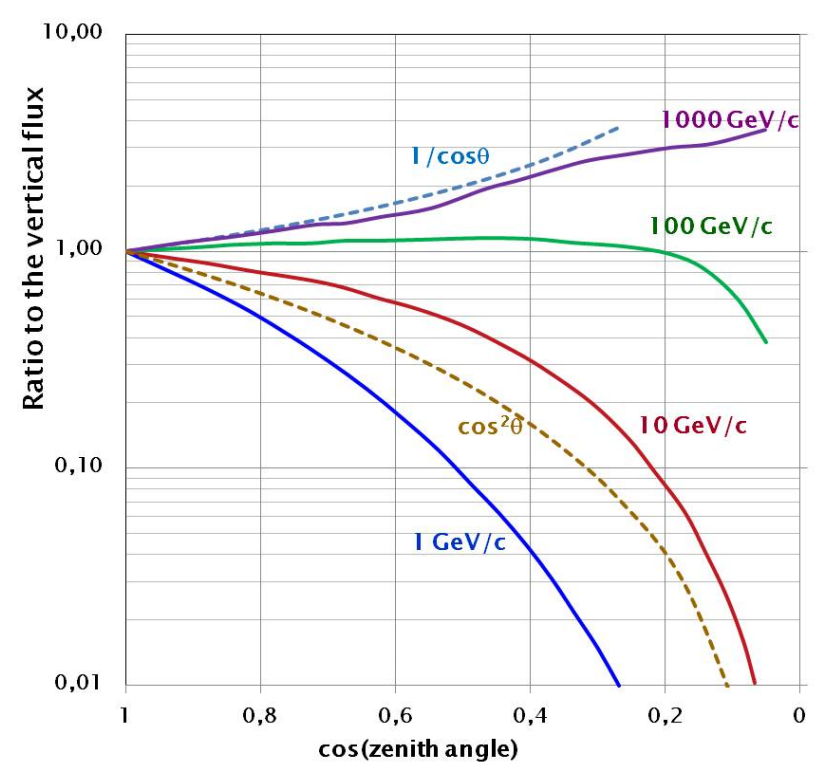
\includegraphics[width=\textwidth]{angular_distribution}
		\caption{\label{fig:angular_distribution}
		Distribuzione angolare dei muoni in funzione dell'impulso
		(distribuzione nell'angolo solido).}
	\end{subfigure}
	\caption{\label{fig:vertical_angular}
	Proprietà dei raggi cosmici al livello del suolo, fonte \cite{1}}
\end{figure}

Il flusso verticale di muoni con energia $E_{\mu} > \SI{1}{\GeV}$ attraverso una superficie orizzontale vale $I_v(E_{\mu} > \SI{1}{\GeV}) \sim \SI{70}{m^{-2} s^{-1} sr^{-1}}$ che corrisponde alla nota stima di una particella per $\SI{}{cm^2}$ per minuto. Se scegliamo un taglio in energia meno rigido, più vicino alle condizioni del nostro esperimento (in cui in pratica il taglio in energia è fatto dal soffitto del laboratorio) otteniamo un flusso $I_v(E_{\mu} > \SI{300}{\MeV}) \sim \SI{100}{m^{-2} s^{-1} sr^{-1}}$.

\paragraph{Distribuzione angolare}

La distribuzione angolare del flusso di muoni in arrivo al livello del mare dipende dall'energia degli stessi come mostrato in Figura~\ref{fig:vertical_angular}\subref{fig:angular_distribution}, questo perché muoni più energetici hanno una vita media più lunga e riescono a viaggiare per distanze maggiori prima di decadere.
La Figura~\ref{fig:vertical_angular}\subref{fig:angular_distribution} mostra che per muoni con impulsi dell'ordine di qualche GeV/c la dipendenza del flusso dall'angolo è $\propto \cos^n\theta$ con $n$ intorno a 2.

La distribuzione angolare del flusso di muoni riveste un ruolo importante nella nostra misura poiché l'apparato non può essere ruotato e gli angoli accettati dipendono dalla geometria dell'apparato. Questo vuol dire che senza conoscere la distribuzione angolare dei raggi in arrivo non ci è possibile ottenere il flusso totale (integrato su tutto l'angolo solido) dei muoni in arrivo. Sapendo che la distribuzione dei muoni è approssimabile con $A_0 \cos^n\theta$ e misurando il flusso con accettanze angolari diverse ci è possibile ricavare sia $A_0$ (il flusso verticale) che $n$.

\paragraph{Risultati precedenti in letteratura}

Il flusso di raggi cosmici, oltre a dipendere dal'altitudine, dipende anche dalla latitudine geomagnetica e varia nel tempo seguendo i cicli solari. Questo rende difficile confrontare misure fatte in luoghi e momenti diversi che quindi hanno una certa variabilità.
In \autoref{tab:letteratura} riportiamo un breve elenco di risultati presenti in letteratura. Nella tabella 3.23 in \cite{7}  è riportato un vasto insieme di misure di flussi verticali integrati di raggi cosmici sul livello del mare.


\begin{table}
	\small
	\hspace{-3em}
	\begin{tabular}{lccccc}
		\hline
		Autori & Lat. [$\SI{}{\degree N}$]& Alt. [$\SI{}{m}$]& Impulso [$\SI{}{Gev/c}$] &$n$ & \makecell{Flusso a $\theta=0$\\{}[$\times 10^{-3}\si{cm^{-2}s^{-1}sr^{-1}}$]}\\
		\hline
		Crookes, Rastin \cite{2} & 53 & 40 &$\ge$ 0.35 &2.16 $\pm$ 0.01 &9.13  $\pm$ 0.12\\
		Greisen \cite{3} \cite{4}& 54 & 259 &$\ge$ 0.33& 2.1 &8.2  $\pm$ 0.1\\
		Judge, Nash \cite{5}& 53 & s.l.m. & $\ge$ 0.7 & 1.96  $\pm$ 0.22 & --\\
		Fukui et al. \cite{6}& 24 & s.l.m.& $\ge$ 0.34 &-- &7.35 $\pm$ 0.2\\
		Gokhale \cite{7}& 19 & 124 &$\ge$ 0.27 &-- &7.55 $\pm$ 0.1\\
		Karmakar et al. \cite{8}& 16 & 122 &$\ge$ 0.353 &2.2 &8.99 $\pm$ 0.05\\
		Sinha, Basu \cite{9}& 12 & 30 &$\ge$ 0.27 &-- &7.3 $\pm$ 0.2\\
		S. Pal \cite{10}& 10.61 & s.l.m. &$\ge$ 0.280 &2.15 $\pm$ 0.01 &6.217 $\pm$ 0.005\\
		Allkofer et al. \cite{11}& 9 & s.l.m. &$\ge$ 0.32 &-- &7.25 $\pm$ 0.1\\
		S. Pethuraja et al. \cite{12}&1.44 & 160 &$\ge$ 0.11 &2.00 $\pm$ 0.18 & 7.0 $\pm$ 0.5\\
		\hline
	\end{tabular}
	\caption{\label{tab:letteratura}
	Misure in letteratura del flusso verticale e della distribuzione angolare di muoni
	a varie latitudini e altitudini.}
\end{table}

\subsubsection{Selezione in impulso}

Stimiamo l'effetto del tetto sulle particelle in arrivo.
In base alla Figura~\ref{fig:vertical_angular}\subref{fig:vertical_flux},
ci concentriamo su muoni ed elettroni.

\paragraph{Muoni}

Per i calcoli sui muoni ci avvaliamo del noto grafico%
\footnote{\emph{Particle Physics Booklet 2014}, pag. 255}
che mostra il rapporto tra percorso residuo e massa della particella in funzione dell'impulso.
Il rapporto percorso residuo/massa corrispondente a muoni di \SI{300}{MeV}
nel piombo è circa \SI{2e3}{g\,cm^{-2}\,GeV^{-1}}.
Per trovare il percorso residuo bisogna moltiplicare questa quantità per la massa della particella
e dividere per la densità del materiale.
Risulta un percorso residuo di \SI{20}{cm}.
Stimiamo che il tetto equivalga a meno di \SI{20}{cm} di piombo,
quindi anche i muoni cosmici meno energetici non vengono fermati.

\paragraph{Elettroni}

La perdita di energia al minimo di ionizzazione è circa \SI{1.5}{MeV\,g^{-1}\,cm^2}.
Quindi, supponendo un soffitto spesso circa \SI{10}{cm} e densità circa \SI{5}{g\,cm^{-3}},
gli elettroni perdono almeno \SI{70}{MeV}.
Guardando Figura~\ref{fig:vertical_angular}\subref{fig:vertical_flux},
vediamo che allora il flusso verticale di elettroni è meno dell'\SI{8}\% di quello dei muoni.


\subsection{Efficienza}

I rivelatori di raggi cosmici di cui disponiamo sono un sistema composto da una lastra di scintillatore plastico, una guida ottica e un fotomoltiplicatore.
Quando una particella attraversa il rivelatore rilascia energia, portando all'eccitazione o ionizzazione gli elettroni del materiale a cui segue l'emissione di fotoni proporzionalmente all'energia rilasciata.
I fotoni prodotti propagano nella guida ottica fino a raggiungere il fotomoltiplicatore dove il segnale viene convertito in un impulso proporzionale alla luce in arrivo.

Le caratteristiche più importanti dei nostri rivelatori sono il rapporto segnale/rumore e l'efficienza.

Per eseguire correttamente la misura finale del flusso di raggi cosmici è fondamentale tenere perfettamente sotto controllo questi due parametri. Buona parte della discussione che seguirà sarà incentrata sull'analisi delle misure preliminari che ci hanno permesso di caratterizzare il nostro apparato di misura in modo da poter progettare nel migliore dei modi la misura di flusso.

Ci aspettiamo che l'efficienza (e conseguentemente il rapporto segnale/rumore) dipenda da molti fattori:
\begin{itemize}
	\item tensione di alimentazione del fotomoltiplicatore;
	\item soglia dei discriminatori;
	\item posizione di incidenza delle particelle sulla lastra;
	\item energia rilasciata dalle particelle;
	\item tempi morti dell'elettronica;
	\item rumori ambientali.
\end{itemize}
Andiamo brevemente ad analizzarli.

\paragraph{Tensione di alimentazione e soglia}
Come già visto nell'esperienza preliminare la tensione di alimentazione e la soglia dei discriminatori sono i due parametri principali su cui possiamo agire per modificare l'efficienza e conseguentemente rapporto segnale/rumore. La prima constatazione che possiamo fare è che i rivelatori presi singolarmente sono molto rumorosi e non è possibile eseguire una misura di flusso senza abbattere il rumore tramite coincidenze. L'uso delle coincidenze abbatte il rumore ma limita e seleziona l'angolo solido sul quale misuriamo il flusso. Notiamo anche che i rivelatori  hanno un comportamento sostanzialmente disuniforme tra di loro per efficienze massime e rapporto segnale/rumore (a pari efficienza).

\paragraph{Efficienza locale}
I fotoni sono emessi isotropi nella posizione in cui la particella attraversa la lastra,
di questi solo una piccola parte raggiunge direttamente il fotomoltiplicatore, il resto in parte raggiunge il PMT dopo essere stato riflesso più volte dalla superficie argentata che avvolge gli scintillatori e nella guida ottica e in parte assorbito. Ci aspettiamo quindi che l'efficienza di rivelazione sia maggiore per le particelle che passano vicine al PMT e non abbiamo motivo di aspettarci un'asimmetria dell'efficienza locale rispetto all'asse di simmetria del rivelatore\footnote{Come vedremo più avanti questa previsione verrà disattesa.}.

\paragraph{Energia rilasciata}
L'efficienza dipenderà dalla quantità di fotoni emessi e quindi dall'energia rilasciata dalle particelle. Come detto precedentemente i muoni (che ci attendiamo siano la gran parte del flusso in arrivo) sono MIP per cui in prima approssimazione rilasciano tutti la stessa quantità di energia per unità di lunghezza attraversata (che dipende dall'angolo di incidenza): in ultima analisi l'efficienza dipenderà dall'angolo di incidenza delle particelle.
Quando mettiamo in coincidenza dei rivelatori stiamo selezionando un certo angolo solido e una certa distribuzione angolare (e della posizione di incidenza) dei raggi in arrivo, per cui l'efficienza varierà al variare delle coincidenze che utilizzeremo.

\paragraph{Tempi morti dell'elettronica}
I tempi morti dell'elettronica sono responsabili di un'inefficienza ineliminabile dei nostri rivelatori e tuttavia spesso sarà necessario aumentare i tempi morti per evitare problemi di retrigger\footnote{Ovvero quando i discriminatori scattano più volte sullo stesso segnale.}. Il tempo morto totale (e quindi l'inefficienza) aumentano all'aumentare del rumore. Questa inefficienza è facilmente tenuta sotto controllo (basta conoscere il rate e misurare il tempo morto) a differenza delle dipendenze prima esposte, per il quale non disponiamo di un modello utilizzabile.

\paragraph{Rumori ambientali}
La luce ambientale che riesce a penetrare l'involucro opaco dei rivelatori può aumentare sensibilmente il rumore dei rivelatori. Per limitare questo effetto bisogna migliorare l'opacizzazione degli stessi e provvedere a schermarli ulteriormente dalla luce ambientale.

La conclusione di queste considerazioni è che l'efficienza è una quantità molto difficile da tenere sotto controllo e conoscere con precisione: in linea di principio quando misuro l'efficienza di un rivelatore (ad esempio con un rapporto di rate tra coincidenze  a 2 e a 3) sto misurando l'efficienza di quella precisa configurazione di lastre.

Per ridurre drasticamente la dipendenza dell'efficienza da tutti questi fattori senza necessariamente tenerli in conto o modellizzarli è necessario tenere l'efficienza intrinseca\footnote{Qui con efficienza intrinseca intendiamo quella scorporata dall'inefficienza dovuta ai tempi morti che non dipende dalla distribuzione angolare e dalla posizione di incidenza dei raggi.} il più possibile vicino al 100\%. Bisognerà però fare attenzione a tenere sotto controllo il rumore.
 
 

\subsection{Geometria}

\begin{figure}
	\center
	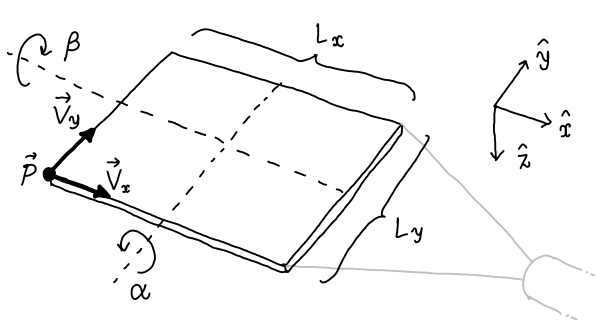
\includegraphics[width=25em]{geometriadef}
	\caption{\label{fig:geometriadef}
	Definizione del modello geometrico.
	Gli angoli $\alpha$ e $\beta$ sono nulli
	quando il lato della lastra ortogonale al loro asse di rotazione è orizzontale.
	Gli assi di rotazione sono riferiti alla lastra.}
\end{figure}

Esponiamo la modellizzazione geometrica dell'apparato ai fini di calcoli e simulazioni
(vedi \autoref{fig:geometriadef}).
Consideriamo ogni lastra di scintillatore come un parallelepipedo.
Teniamo conto dei \emph{disallineamenti} cioè della posizione arbitraria nello spazio delle lastre,
supponendo però che sia poco diversa da quella ideale di lastre orizzontali, rettangolari e allineate verticalmente.
Chiamiamo $x$ la direzione orizzontale parallela ai tubi fotomoltiplicatori,
$y$ quella ortogonale,
$z$ la direzione verticale.
Assumiamo che la direzione verticale data dalla gravità
coincida con la media dei versori normali alle lastre.

\subsection{Calcolo delle coincidenze casuali}

Per tenere conto con simulazioni o calcoli delle coincidenze casuali e dei tempi morti,
trattiamo i segnali digitali come forme perfettamente rettangolari.
Assegniamo la distribuzione esponenziale al tempo tra un \emph{evento} e il successivo.
Un evento genera un fronte di salita%
\footnote{Noi usiamo moduli NIM che hanno logica negativa, quindi un fronte di salita corrisponde in tensione a un fronte di discesa.}
se il tempo trascorso dall'ultimo fronte di salita
è minore del tempo morto.
Il segnale rimane alto per una certa \emph{durata del segnale} fissata.
Il tempo morto è almeno la durata del segnale.
I segnali fanno coincidenza quando sono entrambi alti per almeno un certo \emph{tempo di coincidenza}.

\paragraph{Simulazione Monte Carlo}

Prendiamo un insieme di segnali, indicizzati da $j$,
con rate $r_j$, durate $c_j$ e tempi morti $d_j \ge c_j$.
Per ogni segnale siano $t_{j,i}$ i tempi dei vari eventi.

L'idea di base per simulare le coincidenze è semplice.
Sia $t_{j,i}$ l'ultimo evento che ha generato un fronte di salita sul segnale $j$,
estraiamo $t_{j,i+1}$ dalla distribuzione esponenziale di scala $r_j^{-1}$;
continuiamo a estrarre nuovi eventi finché non superano il tempo morto cioè $t_{j,i+k}>t_{j,i} + d_j$,
allora $t_{j,i+k}$ genera il nuovo fronte di salita.
Generiamo un nuovo fronte sul segnale 0.
Generiamo nuovi fronti sul segnale~1 finché non si verifica che:
o il segnale 1 fa coincidenza con il segnale 0,
o l'ultimo fronte~1 supera l'ultimo fronte 0 abbastanza da non poter fare coincidenze.
Se c'è coincidenza si prosegue generando fronti sul segnale 2;
se alla fine tutti i segnali fanno coincidenza si incrementa il conteggio delle coincidenze.
Si prosegue generando un nuovo fronte sul segnale 0,
finché $t_{0,i}$ non supera il tempo totale.

Questo algoritmo ha il bug che un fronte sul segnale 0 non può generare più di una coincidenza.
La soluzione è la seguente:
si introduce un \emph{segnale leader} $J$ che inizialmente è $J=0$
e che ha il ruolo del segnale 0 nella precedente descrizione.
Quando si verifica una coincidenza,
il nuovo leader è il segnale che ha il fronte di discesa $t_{j,i}+c_j$ maggiore.
Viene aggiunto un nuovo evento al leader solo quando non si verifica una coincidenza.
Il motivo è che qualunque nuova coincidenza
che avvenga senza aggiungere un nuovo evento su un certo segnale,
deve necessariamente avvenire senza aggiungere un evento sul segnale che termina più tardi.


\section{Misura e analisi}

\subsection{Geometria}

\begin{figure}
	\center
	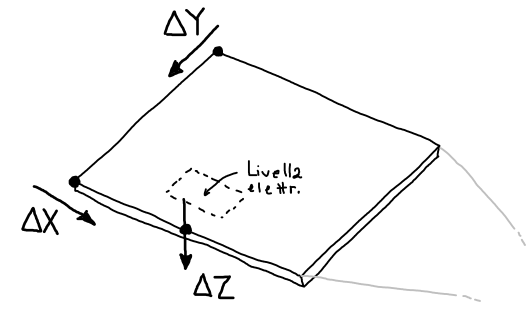
\includegraphics[width=20em]{geometriamis}
	\caption{\label{fig:geometriamis}
	Misura della geometria di una lastra di scintillatore.
	La \emph{profondità} $\Delta Z$ è misurata con il metro a nastro
	con riferimento la lastra più in alto (PM6).
	I \emph{disallineamenti} $\Delta X$ e $\Delta Y$ sono misurati
	con il righello o il metro a nastro usando come riferimento
	una livella a bolla.
	Le \emph{inclinazioni relative} $\alpha_0$ e $\beta_0$ sono misurate con
	una livella elettronica (un cellulare) che ha una risoluzione di \SI{0.1}{\degree}.}
\end{figure}

\begin{table}
	\center
	\begin{tabular}{cccccccc}
		PM & $\Delta X$ [\si{mm}] & $\Delta Y$ [\si{mm}] & $\Delta Z$ [\si{mm}] & $\alpha_0$ [\si\degree] & $\beta_0$ [\si\degree] & $L_x$ [mm]      & $L_y$ [mm]      \\
		\hline
		6  & 0                    & \num{543 \pm 1}      & 0                    & 0.7                     & 0.2                    & \num{400 \pm 2} & \num{482 \pm 1} \\
		5  & \num{-5 \pm 1}       & \num{540 \pm 1}      & \num{102 \pm 1}      & 1.0                     & 0.3                    & \num{404 \pm 2} & \num{482 \pm 1} \\
		4  & \num{1 \pm 1}        & \num{536 \pm 1}      & \num{205 \pm 1}      & 1.2                     & 0.4                    & \num{398 \pm 2} & \num{481 \pm 1} \\
		3  & \num{1 \pm 1.4}      & \num{539 \pm 1}      & \num{308 \pm 1}      & 0.8                     & 0.3                    & \num{400 \pm 2} & \num{480 \pm 1} \\
		2  & \num{2 \pm 1.4}      & \num{531 \pm 1}      & \num{411 \pm 1}      & 0.2                     & 0.6                    & \num{395 \pm 2} & \num{481 \pm 1} \\
		1  & \num{0 \pm 2}        & non mis.             & \num{804 \pm 2}      & 0.8                     & 0.4                    & \num{398 \pm 2} & \num{480 \pm 1}
	\end{tabular}
	\caption{\label{tab:geom}
	Misure di geometria.
	Per gli angoli abbiamo preso un'incertezza pari a metà della risoluzione cioè \SI{0.05}\degree.
	Le incertezze delle misure con righello o metro a nastro
	le abbiamo fissate a una tacca o a due tacche
	a seconda della difficoltà della misura.
	Le misure con incertezza \num{1.4} sono ottenute
	sommando due misure con incertezza \num{1}.
	Per il $\Delta Y$ non misurato,
	prendiamo la media degli altri $\Delta Y$ come valore nominale
	e la deviazione standard campione come incertezza.}
\end{table}

Dobbiamo misurare le caratteristiche geometriche dell'apparato
per assegnare misure alle variabili del modello in \autoref{fig:geometriadef}.

Con una livella a bolla controlliamo che tutte le lastre siano orizzontali.
La livella a bolla ha, per verifica empirica, una risoluzione minore di quella
elettronica del cellulare (\SI{0.1}{\degree}).
Tuttavia la livella elettronica non ha uno zero fisso; lo zero va impostato
appoggiandola su una superficie di riferimento.
Allora misuriamo l'inclinazione delle lastre con la livella elettronica 
(gli angoli di Eulero del cellulare forniti dal software, che chiamiamo $\alpha_0$ e $\beta_0$),
e poi assumiamo, come detto nella \autoref{sec:teogeom},
che l'inclinazione media delle lastre sia nulla.
Questo ci permette di valutare in modo quantitativo quantomeno l'incertezza
dovuta all'inclinazione relativa delle lastre.

Misuriamo la posizione spaziale usando righello, metro a nastro e livella a bolla.
Facendo riferimento alla \autoref{fig:geometriamis} per la notazione, riportiamo
in \autoref{tab:geom} le misure.

Riportiamo le formule per passare dalle misure al modello.
Per convertire le inclinazioni relative in assolute,
sapendo che gli angoli sono piccoli, facciamo direttamente la media sugli angoli:
\begin{align*}
	\alpha &= \alpha_0 - \langle\alpha_0\rangle, \\
	\beta  &= \beta_0  - \langle\beta_0\rangle.
\end{align*}
I parametri di una lastra (equazione \ref{eq:lastra}) sono dati da
\begin{align*}
	\hat V_x &= \begin{pmatrix}
		\cos\alpha, & 0, & \sin\alpha
	\end{pmatrix} \\
	\hat V_y &= \begin{pmatrix}
		\sin\alpha\sin\beta, & \cos\beta, & -\sin\beta
	\end{pmatrix} \\
	\vec P &= \begin{pmatrix}
		\Delta X, & \Delta Y - L_y(\hat V_y\cdot\hat y), & -\Delta Z - \frac12 L_x(\hat V_x\cdot\hat z)
	\end{pmatrix},
\end{align*}
dove abbiamo posto che i lati ``$x$'' delle lastre siano sul piano $xz$; i calcoli trigonometrici sono al secondo ordine in $\alpha$, $\beta$.

\subsubsection{Incertezza dell'accettanza}
\label{sec:uncgeom}

Nell'integrale Monte Carlo \eqref{eq:accmc} per l'accettanza,
le misure di geometria entrano nei termini $w_i(L)$.
Il risultato ha quindi non solo l'incertezza intrinseca del calcolo Monte Carlo,
ma anche un'incertezza associata alle misure di geometria.

Per stimarla procediamo in questo modo:
fissiamo le estrazioni dei raggi con cui calcoliamo l'integrale.
Estraiamo delle misure di geometria pseudocasuali,
usando delle gaussiane con medie i valori nominali e deviazioni standard le incertezze
riportati nella \autoref{tab:geom}.
Calcoliamo $\hat Q$ per ogni estrazione di geometria e, come incertezza geometrica,
prendiamo la deviazione standard campione di questi $\hat Q$
(e la covarianza campione nel caso di più accettanze).
Come valore nominale per $\hat Q$ prendiamo quello calcolato con i valori nominali delle misure di geometria.



\subsection{Configurazione utilizzo ADC}
% troppo giornalistico?  (mi riferisco alla mancanza di articoli)

\begin{figure}
	\centering
	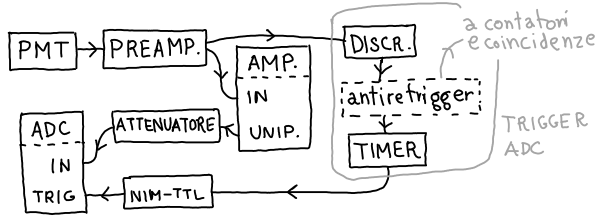
\includegraphics[width=28em]{schemaadc}
	\caption{\label{fig:schemaadc}
	Circuito per misurare l'energia rilasciata negli scintillatori.}
\end{figure}

\marginpar{Cambiare titolo in ``Misura del rilascio di energia''?}
La necessità di misurare quantitativamente il rilascio di energia nel rivelatore ci obbliga ad aggiungere nel nostro crate 3 moduli che permettono di digitalizzare l'uscita del PMT: il preamplificatore, l'amplificatore e l'ADC
(vedi circuito in \autoref{fig:schemaadc}).
Il preamplificatore ha il compito di allungare la durata dell'output del PMT dai nanosecondi ai microsecondi, in modo che l'amplificatore e l'ADC abbiano il tempo di leggerla. Esso è collegato direttamente al PMT che vogliamo usare per evitare riflessioni e non è possibile operare un adattamento di impedenza, in quanto il preamplificatore necessita di un'elevata impedenza d'ingresso per allungare la durata del segnale. 
Il~preamplificatore restituisce un segnale con una salita praticamente istantanea
ed una discesa esponenziale con un $\tau\approx\SI{15}{\mu s}$.

Il compito dell'amplificatore è intensificare il segnale al suo ingresso
(in questo caso quello del preamplificatore)
e restituire un'uscita analogica proporzionale all'energia del segnale in ingresso.
Ci sono due uscite analogiche che generano una forma diversa di segnale,
dette \emph{unipolare} e \emph{bipolare}.
Il manuale specifica che la forma dell'uscita unipolare
è data dalla funzione $e^{-3t}\sin^4{t}$ (simile a una gaussiana), in cui $t$ è il tempo.
La forma bipolare è simile ma ha il massimo anticipato rispetto a quello dell'unipolare.
La tensione massima in uscita è \SI{11}{V}.

Lo scopo dell'ADC è trasformare un segnale analogico in uno digitale
in modo che questo possa essere salvato su un computer.  
La conversione del segnale parte dopo circa \SI{1}{\micro s} dall'arrivo di un segnale di \emph{trigger} e dura all'incirca tale intervallo di tempo. L'ADC può leggere segnali analogici che vanno da qualche \si{mV} a \SI{3.3}{V} e può digitalizzarne al massimo 40 al secondo;
il trigger legge un segnale TTL a~\SI{3.3}{V}.

Per poter sfruttare l'apparato di digitalizzazione dobbiamo trasformare l'uscita del PMT adoperando il preamplificatore,
attenuare il segnale dell'amplificatore in modo che non possa danneggiare l'ADC
e costruire un trigger che faccia partire l'acquisizione
in modo che l'ADC campioni il segnale sul massimo dell'uscita dell'amplificatore.
Per fare il trigger mettiamo un discriminatore sull'uscita del preamplificatore
e la ritardiamo con un timer.

\subsubsection{Taratura del trigger}

\begin{figure}
	\centering
	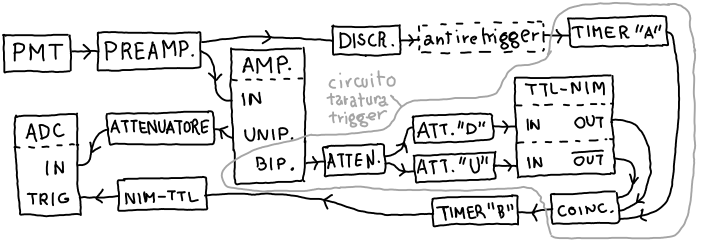
\includegraphics[width=0.9\textwidth]{schematrig}
	\caption{\label{fig:schematrig}
	Circuito per la taratura del timer del trigger dell'ADC.
	Il timer~A è regolato in modo che la coincidenza possa scattare
	solo in un certo istante del segnale in uscita bipolare dell'amplificatore.
	L'istante è stato scelto in modo da avere la massima pendenza del segnale
	per restringere la durata del segnale in uscita del discriminatore a doppia soglia.
	Per lo stesso motivo usiamo il bipolare anziché l'unipolare (ha una pendenza maggiore).
	Per eseguire la taratura modifichiamo la durata del timer~B
	cercando di massimizzare la lettura dell'ADC.
	Per tornare al circuito di misura (\autoref{fig:schemaadc}),
	togliamo la parte di taratura e colleghiamo in serie i timer A e B.}
\end{figure}

\marginpar{Aggiungere ``dell'ADC'' al titolo?}
La documentazione a disposizione dell'ADC non specifica esattamente
quanto tempo intercorre tra il segnale di trigger e il campionamento.
Per regolare il timer del circuito di trigger usiamo un circuito ausiliario
(vedi \autoref{fig:schematrig}).
L'idea è mandare in ingresso all'amplificatore segnali ad energia costante
e poi regolare la durata del timer del trigger massimizzando la lettura dell'ADC,
poiché dobbiamo campionare sul massimo.
Poiché la forma del segnale in ingresso influisce sull'allineamento temporale
dell'uscita con l'ingresso,
per essere sicuri di tarare correttamente il trigger
dobbiamo mandare in ingresso proprio i segnali che dobbiamo misurare.%
\footnote{Quindi, per esempio, non possiamo usare un impulsatore.}
Quindi, per avere segnali ad energia costante,
selezionamo direttamente i segnali in base all'uscita dell'amplificatore.
Vogliamo avere un discriminatore a doppia soglia%
\footnote{Discriminatore che ha uscita a livello alto quando la tensione in ingresso è compresa tra le due soglie.}
sull'uscita dell'amplificatore, con soglie piuttosto vicine,
in coincidenza con un timer ausiliario per leggere l'uscita dell'amplificatore
sempre nello stesso punto della forma del segnale.
Poiché non disponiamo di moduli in logica positiva,
costruiamo questo discriminatore sfruttando il fatto che il modulo \texttt{TTL-NIM}
non è altro che un discriminatore dove la soglia (positiva) è quella che distingue i livelli logici.
Per avere due soglie diverse
usiamo due attenuatori impostati con una differenza di attenuazione più piccola possibile.
\marginpar{Forse dobbiamo parlare qui del problema che il nostro trigger non è detto
triggeri come triggera l'amplificatore (da cui la foto incriminante).}



\subsection{Effetto del materiale sulla misura}

Abbiamo testato quanto la presenza di lastre di piombo potesse influire sulla rivelazione dei raggi cosmici. Abbiamo a disposizione il seguente materiale:
\begin{itemize}

\item 3 lastre rigide di piombo\\
spessore=\SI{4\pm1}{mm}\\
L1=\SI{39.9\pm0.1}{ cm}\\
L2=\SI{40.0\pm0.1}{cm}

\item 1 lastra di alluminio con le stesse dimensioni delle 3 precedenti

\item 10 lastre flessibili di piombo\\
spessore=\SI{2\pm1}{ mm}\\
L1=\SI{47.5\pm0.1}{ cm}\\
L2=\SI{45.0\pm0.1}{ cm}

\end{itemize}

\subsubsection{Conteggi}

Abbiamo posizionato le lastre rigide tra il PM3 ed il PM4 per vedere se esse riuscivano a fermare parte dei muoni. Per fare questa misura abbiamo confrontato le coincidenze  PM5 \& PM4 e PM5 \& PM4 \& PM3, però non possiamo confrontarle così come sono a causa dell'accettanza geometrica: anche in assenza delle lastre le coincidenze a tre sono diverse da quelle a due. Allora correggiamo le coincidenze a due con un Monte Carlo che tiene in considerazione le efficienze dei tre rivelatori. Il fattore di correzione ottenuto è il rapporto tra le accettanze delle due configurazioni  $\delta=mc(\text{PM5 \& PM4 \&PM3})/mc(\text{PM5 \& PM4})=65.71\pm0.02\%$, dove $mc$ indica il risultato del Monte Carlo per la configurazione in questione. Siano $C2$ il numero di coincidenze a due e $C3$ il numero di quelle a tre, per capire quanto sia significativo l'effetto delle lastre sulle nostre misure confrontiamo le quantità $C2'=C2 \cdot \delta$ e $C3$ in funzione del numero di lastre inserite%
\footnote{Nel grafico di \autoref{cfr} non è presente il caso di 3 lastre perché, avendone una di alluminio, abbiamo deciso di metterla insieme alla terza lastra di piombo.}. %
Dal confronto, presente in \autoref{cfr}, non si evince nessuna differenza tra i conteggi a meno di una separazione di $3\sigma$ nell'ultimo caso che, come descritto nella sezione successiva, rappresenta solo una fluttuazione.
\marginpar{scrivere il tempo di misura || $3\sigma$ l'ho detto ad occhio || giustificazione nella sezione successiva || efficienze}

\begin{figure}[h]
\centering
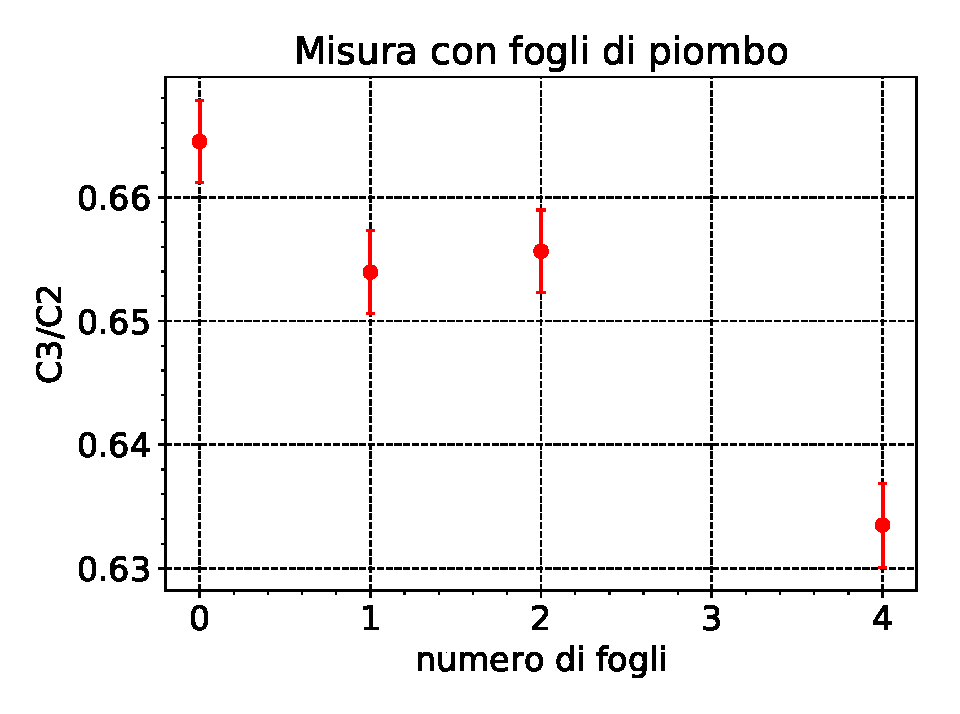
\includegraphics[width=8 cm]{confronto}
\caption{Confronto tra le coincidenze a due corrette e quelle a tre in funzione del numero di lastre inserite sul PM3.}
\label{cfr}
\end{figure}

\subsubsection{Energia}

\begin{huge}
QUI CI SAR\`A DA SCRIVERE IL VERGOGNOSO FALLIMENTO DELL'ADC
\end{huge}

Infine abbiamo eseguito due acquisizioni di lunga durata. Nella prima abbiamo messo tutte le lastre a nostra disposizione sul PM1 e abbiamo acquisito i loro rilasci di energia per tutta la notte. Il giorno seguente le abbiamo tolte ed abbiamo preso dati per \SI{4}{ore}. In entrambi i casi il trigger dell'ADC è dato dalle coincidenze PM2 \& PM1.  Abbiamo normalizzato 
\marginpar{dire che Python divide per l'area o si capisce?\\
\emph{Bisogna scriverlo anche nella caption, anche la label dell'asse $y$ è da cambiare.}}
entrambi gli spettri per poterli confrontare ed evincere che non mostrano nessuna differenza, come si può vedere in \autoref{gemini}. \marginpar{non ci sono le barre d'errore sulle barre dell'istogramma\\
\emph{Non si vedrebbero credo. In questo caso un confronto quantitativo andrebbe fatto con una qualche statistica.}}

\begin{figure}[h]
\centering
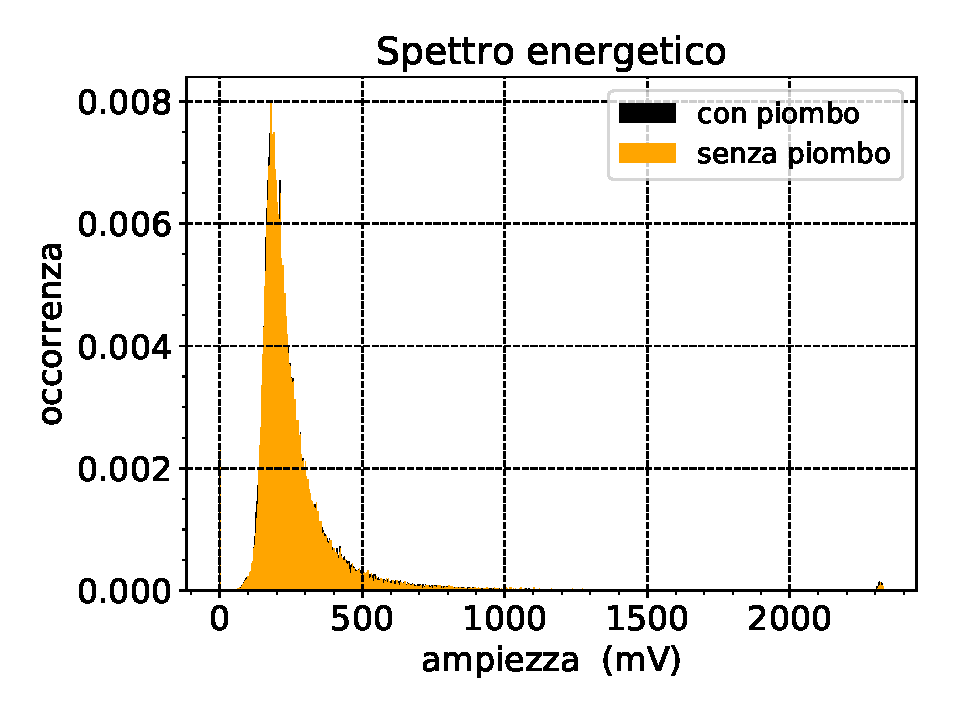
\includegraphics[width=8 cm]{gemelli}
\caption{Confronto tra gli spettri normalizzati con e senza piombo. Il picchetto a destra è dato dagli eventi talmente energetici da saturare l'uscita dell'amplificatore.}
\label{gemini}    
\end{figure}

\marginpar{solo a me la legenda fa pensare alla benzina?}



\subsection{Lunghezza di attenuazione}

La possibilità di fare misure locali con il miniscint 
\marginpar{dobbiamo chiamarlo miniscint?}
ci permette di misurare la lunghezza di attenuazione del sistema scintillatore più guida di luce. Avendo preso misure soltanto sullo scintillatore potrebbe sembrare che abbiamo misurato soltanto la sua lunghezza di attenuazione, ma la nostra strumentazione rivela un evento soltanto quando i fotoni rilasciati raggiungono il PMT dopo aver attraversato la guida di luce. 
Abbiamo eseguito le misure dividendo il PM1 in 16 caselle e ponendo su ognuna di esse il miniscint nei punti mostrati in \emph{figura}. 
\marginpar{inserire disegno, descrizione e dimensioni miniscint}

Nel fare le misure sulle caselle periferiche abbiamo appoggiato il miniscint sulla struttura che circonda il PM1 in modo che l'angolo tra esso ed il miniscint sia sempre lo stesso. Tale accorgimento ci permette di usare quelle misure per stimare l'efficienza locale (relativa) del PM1 \emph{che sarà trattata in dettaglio in una delle sezioni seguenti  (dire quale) }.                            \marginpar{spiegare quel ``relativa'' nella relazione completa}
Per ogni casella abbiamo acquisito il numero di coincidenze verificatesi in \SI{1000}{s}. Al PM1 era collegata l'ADC in modo da poter registrare anche il rilascio di energia in ogni sezione.

Se chiamiamo $N$ il numero di muoni che attraversano ogni casella, possiamo legare questa quantità alla lunghezza di attenuazione attraverso la relazione \eqref{exp} in cui $x$ è la distanza orizzontale del miniscint dalla guida di luce; $N_0$ e $\lambda$ sono i parametri del fit. 
\begin{equation}
N=N_0 e^{-\frac{x}{\lambda}}  \label{exp}
\end{equation}

I dati raccolti sono stati trattati in due modi diversi perché entrambi permettono di ricavare la lunghezza di attenuazione e nessuno dei due ha delle caratteristiche che lo rendono preferibile rispetto all'altro.

\subsubsection{Media per colonne}

La prima strategia di analisi dati consiste nel fare la media dei conteggi per ognuna delle 4 colonne e poi fittare questi punti con la funzione \eqref{exp}.
Il fit ha restituito i seguenti risultati: $N_0=634\pm25$,  $\lambda=\SI{118\pm32}{cm}$, $\chi^2=11\pm2$ con dof=2 e covarianza normalizzata corr$(N_0,\lambda)=-0.8$. 
La \autoref{atte} mostra le medie ottenute e la relativa funzione di fit.
\begin{figure}[h]
\centering
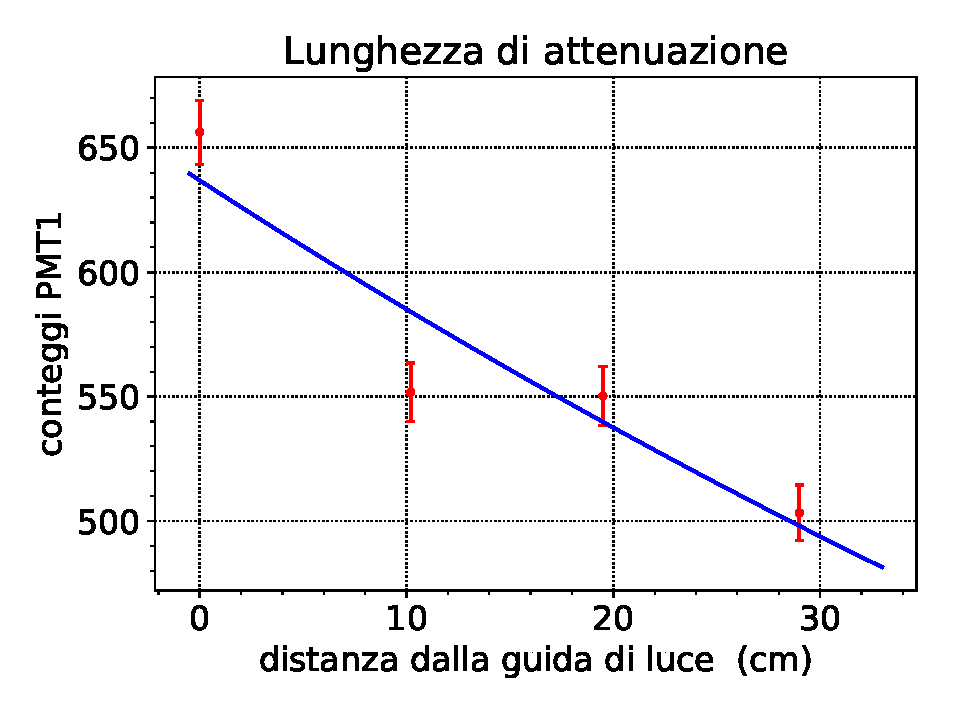
\includegraphics[width=8 cm]{atte}
\caption{Fit relativo alla lunghezza di attenuazione calcolata facendo la media per colonne.}
\label{atte}
\end{figure}

\begin{table}[h]
\centering
\begin{tabular}{| c | r @{$\pm$} l |}
\hline
colonna & \multicolumn{2}{c|}{media} \\
\hline
D & 503&11 \\
C & 550&12 \\
B & 551&12 \\
A & 656&13 \\
\hline
\end{tabular}
\caption{Dati del grafico in \autoref{atte}. La colonna D è quella più lontana dalla guida di luce.}
\end{table}

\subsubsection{Media per righe}

La seconda strategia adottata consiste nel fittare con la \eqref{exp} i conteggi di ogni riga separatamente e poi fare la media delle 4 lunghezze di attenuazione ottenute.
In \autoref{4atte} è possibile vedere le 4 curve con le relative funzioni di fit, mentre la \autoref{tab:righe} contiene i risultati del fit.

\begin{table}[h]
\centering
\begin{tabular}{| c | r @{$\pm$} l  | r @{$\pm$} l  | c |}
\hline
riga & \multicolumn{2}{c|}{$N_0$} & \multicolumn{2}{c|}{ $\lambda$ [\si{cm}] } & $\chi^2$ \\
\hline
1 & 711&19 & 121&23 & 1\\
2 & 638&32 & 127&47 & 4\\
3 & 632&60 & 73&30 & 15\\
4 & 565&21 & 228&111 & 2\\
\hline
\end{tabular}
\caption{Risultati restituiti dai fit presenti in \autoref{4atte} riga per riga. Tutti i fit hanno 2 gradi di libertà.}
\label{tab:righe}
\end{table}


La media dei parametri del fit restituisce $\langle\lambda\rangle=\SI{110\pm17}{cm}$ e $\langle N_0\rangle=643\pm13$.
\begin{figure}[h]
\centering
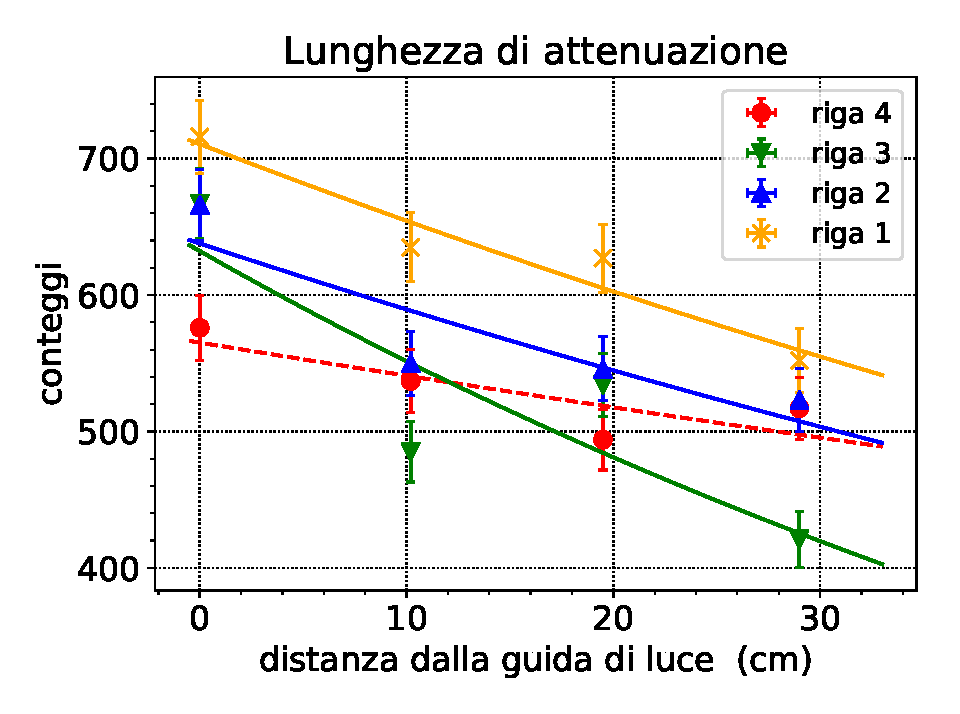
\includegraphics[width=8 cm]{4atte}
\caption{Fit relativo alla lunghezza di attenuazione calcolata facendo la media per righe. Il numero delle righe è quello indicato dalla figura \emph{autoref(schema)}.}
\label{4atte}
\end{figure}


\subsubsection{Limiti della misura}

I parametri ricavati dai 2 fit precedenti sono compatibili ed hanno un errore maggiore del 10\%. Con la strumentazione a nostra disposizione non è possibile determinare la lunghezza di attenuazione con maggiore precisione. Innanzitutto abbiamo usato un miniscint con un'area di \SI{14.7\pm0.9}{cm^2} la cui parte scintillante era appoggiata sul PM1 e la sua cassa \marginpar{``cassa'' va bene?} era appoggiata sulla struttura di metallo che lo circondava. L'angolo formato tra i due scintillatori per le misure periferiche è stato misurato e vale \SI{12.7\pm0.1}{\degree}, invece assume valori ogni volta diversi per le misure nelle altre caselle. Questo implica che l'area sottesa dal miniscint è maggiore di quella della sua parte scintillante e proprio per questo abbiamo deciso di non infittire la griglia disegnata sul PM1, considerando ogni casella di essa come l'area in cui si sarebbero misurate gran parte delle coincidenze. A questo effetto si aggiunge lo spessore del miniscint che vale all'incirca \SI{1}{cm} e può far scattare coincidenze anche quando un muone passa al di fuori della casella in cui il miniscint è stato posizionato. Questa evenienza diventa ancora più frequente quando il miniscint è inclinato perché, essendo in parte sollevato, permette ai muoni che lo hanno attraversato con angolo maggiore di giungere in un punto ancora più lontano della lastra sottostante. In questo caso lo spessore del miniscint può soltanto amplificarne l'effetto, in quanto se fosse inclinato con un angolo sufficientemente elevato riuscirebbe a intercettare sempre meglio  i muoni a grande angolo a discapito di quelli a piccolo angolo.
Le dimensioni trasversali del miniscint non permettono di definire la distanza dalla guida di luce meglio del loro valore e sappiamo anche che i fotoni, per arrivare al fotomoltiplicatore,  non percorrono una linea retta, ma vengono riflessi dal materiale che compone la lastra dello scintillatore e la guida di luce (riflessione totale) oppure dalla carta argentata che riveste gli stessi. Percorrendo queste traiettorie vengono attenuati ulteriormente e non abbiamo nessuna informazione su come essi arrivino al PMT1 né in linea di massima né caso per caso.

\subsubsection{Lunghezza di attenuazione in energia.}

Abbiamo analizzato i dati registrati dall'ADC collegata al PM1 (\autoref{fall}) facendo la media dei rilasci di energia per ogni colonna ma non abbiamo potuto estrarne alcuna informazione.
\marginpar{inventare una scusa}
\begin{figure}[h]
\centering
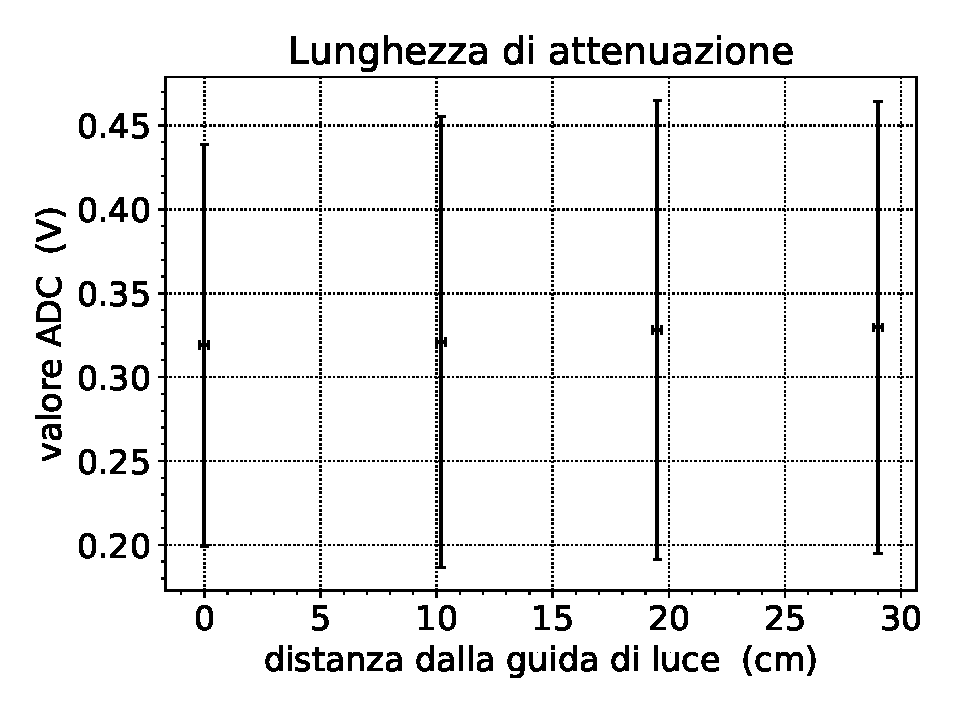
\includegraphics[width=8 cm]{fallimento}
\caption{Energia media giunta al pmt per ogni colonna.}
\label{fall}
\end{figure}



\subsection{Efficienza locale}
\label{localis}
Utilizzando gli stessi dati della \autoref{attenu}, abbiamo studiato le variazioni di efficienza in vari punti del PM1. In \autoref{capolavoro} è presente un grafico 3D che mostra i conteggi ottenuti in ogni casella in cui è stato posizionato il miniscint. Si può apprezzare una diminuzione dei conteggi tra le varie colonne per i motivi discussi in \autoref{attenu} ma è anche evidente come all'interno di una stessa colonna ci siano delle variazioni significative tra una riga e l'altra.
\marginpar{Non so cosa scrivere. Se lo sapete scrivetelo. Io intanto lavoro su altro.}

Per meglio comprendere la situazione, dividiamo tutti i conteggi per quello più alto,
in modo da vedere le variazioni percentuali tra una casella e l'altra del PM1.
La \autoref{auto} riporta i valori dei singoli punti con il loro errore.

\begin{figure}[h]
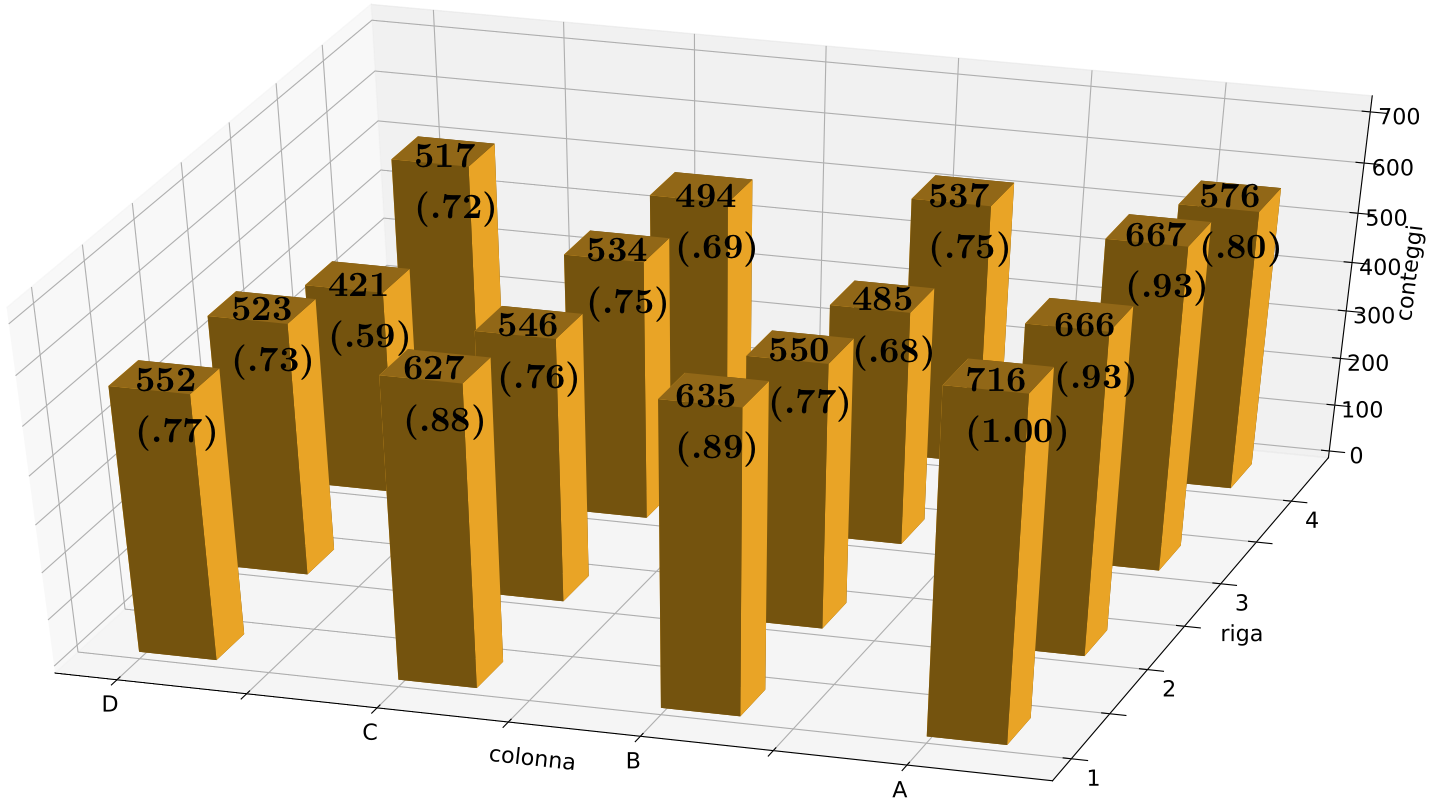
\includegraphics[width=\textwidth]{3d_grande}
\caption{Conteggi PM1 nelle rispettive caselle. L'errore su ogni conteggio è la radice quadrata dello stesso.}
\label{capolavoro}
\end{figure}

\begin{table}[h]
\centering
\begin{tabular}{|c|c|c|c|c|}
\hline
colonna & D & C & B & A \\
 \hline
riga  & & & &  \\
1 &  $ 0.77 \pm 0.04 $ & $ 0.88 \pm 0.05 $ & $ 0.89 \pm 0.05 $ & $ 1 \pm 0 $ \\ 
2 &  $ 0.73 \pm 0.04 $ & $ 0.76 \pm 0.04 $ & $ 0.77 \pm 0.04 $ & $ 0.93 \pm 0.05 $ \\ 
3 &  $ 0.59 \pm 0.04 $ & $ 0.75 \pm 0.04 $ & $ 0.68 \pm 0.04 $ & $ 0.93 \pm 0.05 $ \\ 
4 &  $ 0.72 \pm 0.04 $ & $ 0.69 \pm 0.04 $ & $ 0.75 \pm 0.04 $ & $ 0.80 \pm 0.05 $ \\
\hline 
\end{tabular}
\caption{conteggi normalizzati nelle varie caselle del PM1.}
\label{auto}
\end{table}


\subsection{Rilascio di energia e angolo}   % titolo provvisorio

\begin{figure}
	\centering
	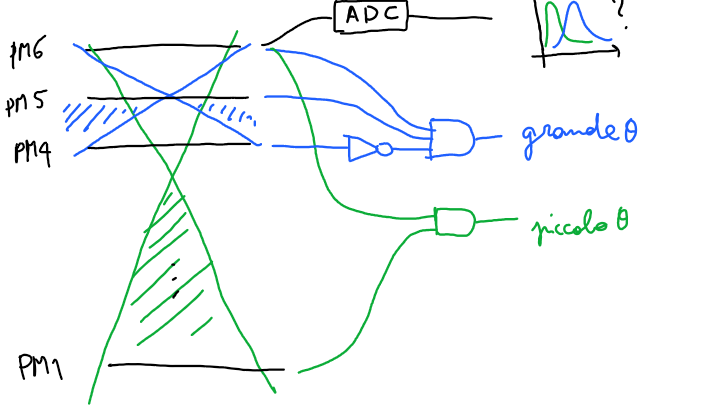
\includegraphics[width=24em]{ang}
	\caption{Schema della strategia di coincidenze per selezionare l'angolo delle particelle incidenti.}
	\label{ang}
\end{figure}

\begin{figure}
	\centering
	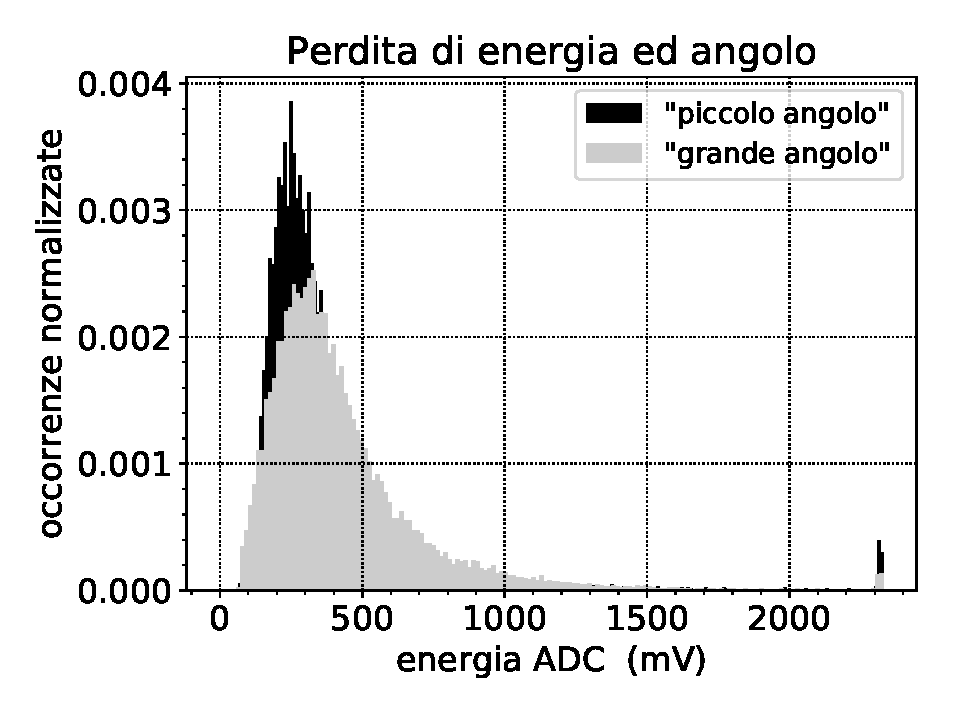
\includegraphics[width=10 cm]{angoli}
	\caption{Energia rilasciata per due selezioni angolari dei raggi significativamente diverse.
	Il picco presente sulla coda è causato dagli eventi abbastanza energetici da saturare l'uscita dell'amplificatore.}
	\label{isto}
\end{figure}

La perdita di energia di una particella carica all'interno di un materiale dipende anche dalla distanza percorsa in esso.
Nel nostro caso è l'angolo di incidenza a stabilire quanta strada farà una particella nella lastra di scintillatore plastico. Per valutare l'entità di questo effetto abbiamo operato nel seguente modo: sfruttando l'ADC misuriamo l'energia persa nell'attraversare la lastra del PM6 selezionando particelle che incidono a ``grande angolo'' oppure a ``piccolo angolo''.
Per selezionare le particelle a piccolo angolo misuriamo le coincidenze PM1 \& PM6, per fare l'opposto contiamo le particelle che soddisfano la configurazione PM6 \& PM5 \& $\neg$PM4.
La \autoref{ang} illustra la strategia di misura. Ci aspettiamo che le particelle che incidono con angolo maggiore perdano più energia, quindi il loro spettro sarà spostato a destra.

Questo è ciò che abbiamo effettivamente verificato.
Infatti la moda per la distribuzione a grande angolo è $\SI{307\pm7}{mV}$,
mentre quella per angoli piccoli vale $\SI{250\pm5}{mV}$.
La moda è calcolata prendendo il massimo dei bin dell'istogramma e assegnando come incertezza la semilarghezza del bin.
In \autoref{isto} sono presenti gli istogrammi ottenuti dalle due configurazioni di misura.



\subsection{Segnale e rumore}
\label{cenno}

\begin{figure}
	\centering
	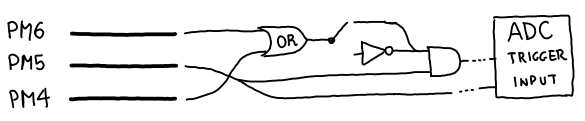
\includegraphics[width=28em]{anti_prov}
	\caption{schema dei collegamenti utilizzati rispettivamente per le misure in coincidenza ed anticoincidenza.}
	\label{anti_prov}
\end{figure}

\begin{figure}
	\hspace{-2cm}
	{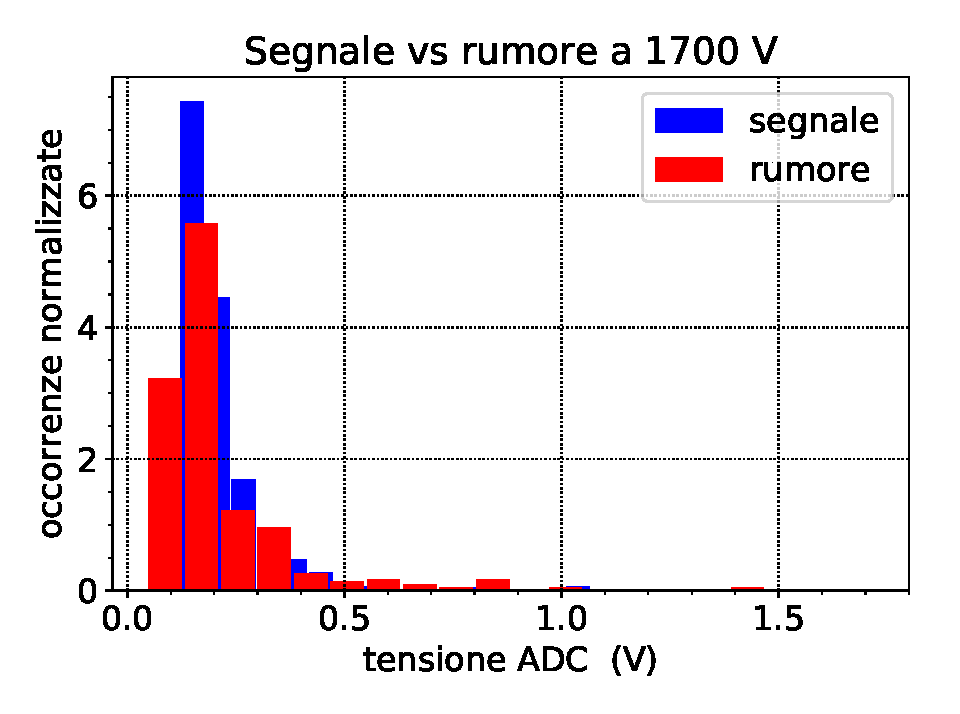
\includegraphics[width=8 cm]{1700}}
	\qquad
	{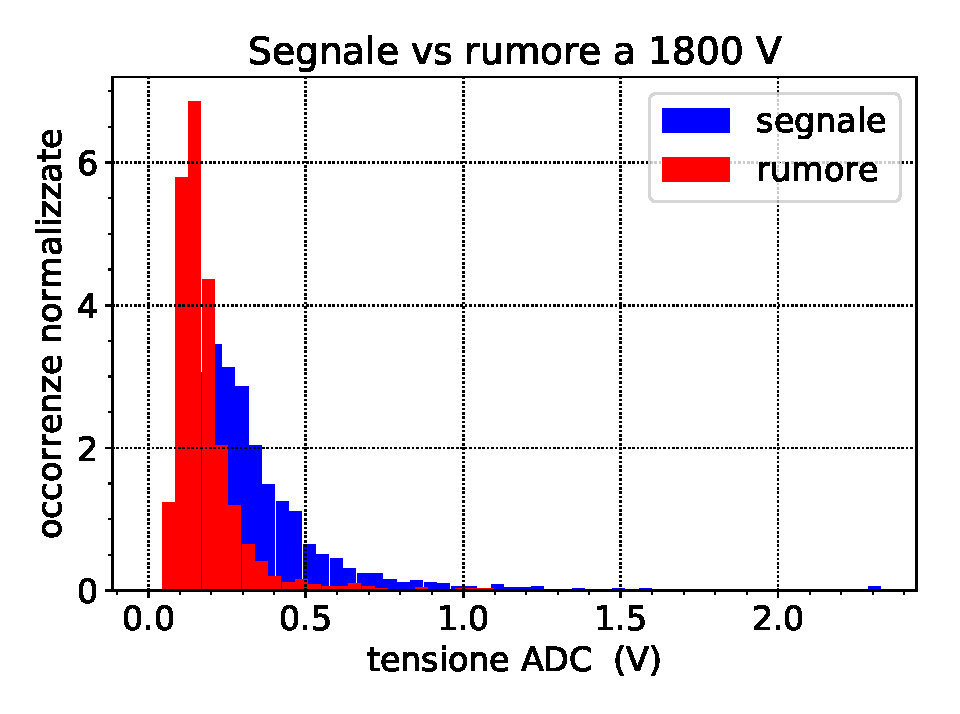
\includegraphics[width=8 cm]{1800}} 

	\hspace{-2cm}
	{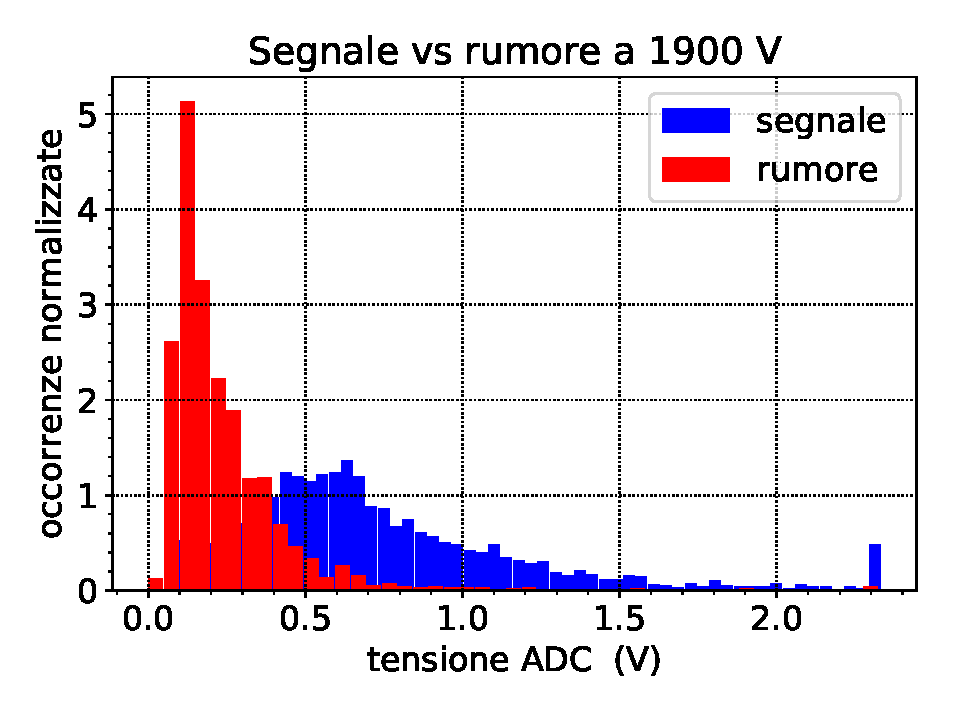
\includegraphics[width=8 cm]{1900}}
	\qquad
	{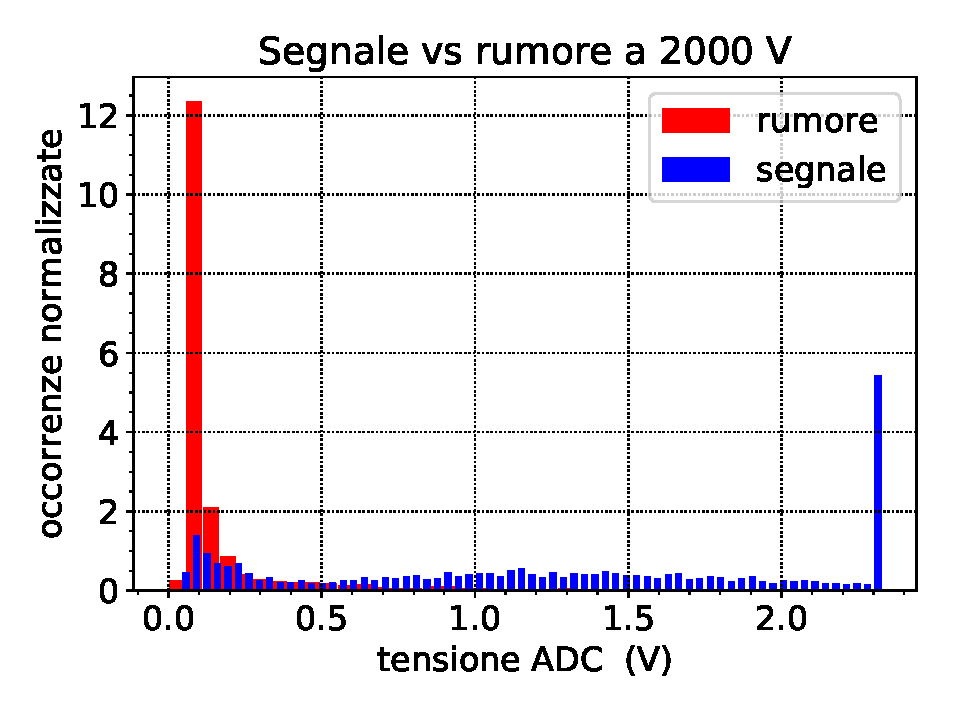
\includegraphics[width=8 cm]{2000}}
	\caption{Istogrammi che rappresentano il variare degli spettri di segnale e rumore per le tensioni più significative.
	A \SI{2000}V sulla sinistra si può notare un picco del segnale nella regione ad alto rumore.}
	\label{quattro}
\end{figure}

Analizziamo lo spettro in energia rilasciata del segnale e lo confrontiamo con quello del rumore.
Per fare questa misura usiamo le espressioni logiche mostrate in \autoref{anti_prov}
misurando il rilascio di energia sul PM5:
per selezionare il rumore usiamo l'espressione $\neg$(PM6 | PM4) \& PM5
in modo da avere la maggior esclusione angolare dei raggi%
\footnote{Non c'è nessun modo di escludere i raggi che passano a $\theta$ abbastanza grande.};
per selezionare il segnale usiamo l'espressione corrispondente a quella del rumore cioè (PM6 | PM4) \& PM5
per minimizzare ulteriori possibili differenze tra le misure
e per poter fare la misura senza cambiare circuito.

Abbiamo acquisito i dati in entrambe le configurazioni spazzando
l'alimentazione del PMT5 da \SI{1600}{V} a \SI{2000}{V} con un intervallo di \SI{50}{V}.
I PM4 e PM6 avevano soglie a \SI{200}{mV} e alimentazione a \SI{1900}V.
In \autoref{quattro} mostriamo un campione significativo delle misure.

Particolare attenzione merita il confronto tra segnale e rumore
per una tensione di alimentazione del PM5 di \SI{2000}{V} (vedi \autoref{quattro}):
segnale e rumore sono molto distinti, ma nell'istogramma del segnale si nota un picco nella regione ad elevato rumore.
Esso comprende circa il \SI{15}\% di tutti gli eventi
ed è di molto superiore al rate di coincidenze casuali attese che,
in tutte le misure, ammontano a meno dell'1\%.


\subsection{Particelle doppie}

\begin{figure}
	\centering
	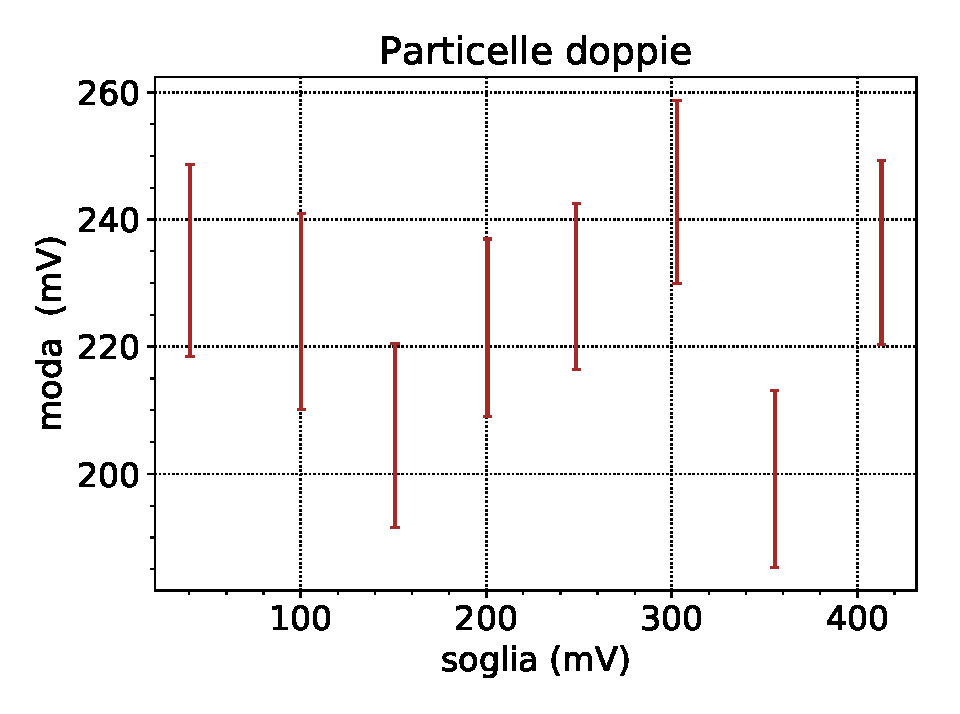
\includegraphics[width=23em]{doppie}
	\caption{Moda della distribuzione del rilascio di energia nel PM5
	negli eventi in coincidenza PM4 \& PM5
	in funzione della soglia del PM4.}
	\label{corre}
\end{figure}

\begin{figure}
	\centering
	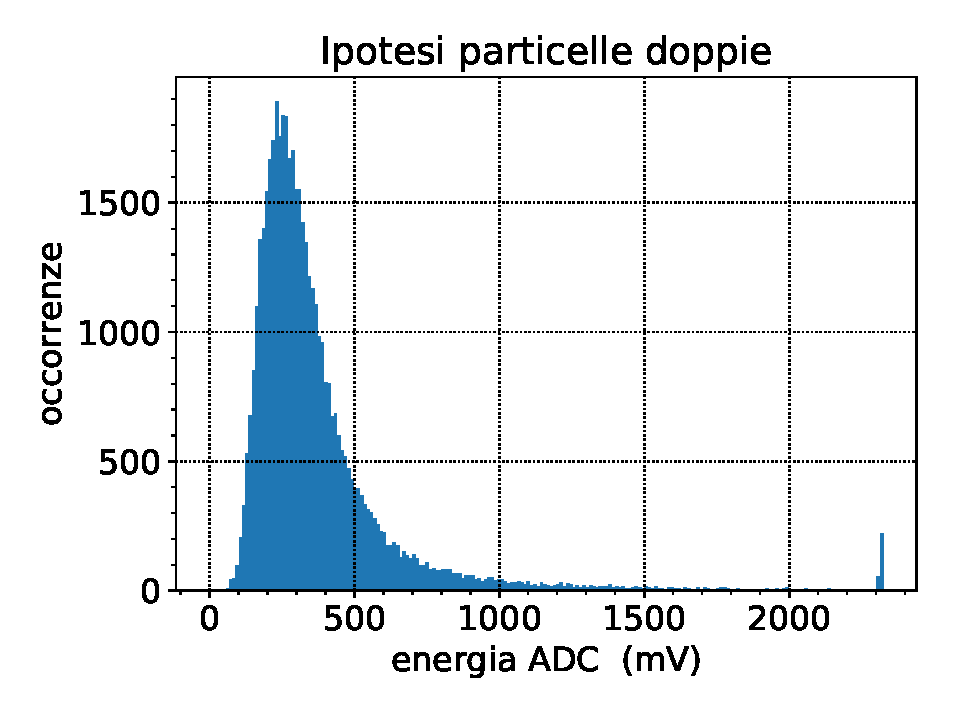
\includegraphics[width=23em]{nuovo}
	\caption{Spettro dei rilasci per la configurazione 1\&6. La distribuzione è chiaramente unimodale.}
	\label{nuovo}
\end{figure}

Ci aspettiamo di osservare una distribuzione del rilascio di energia bimodale,
con una moda circa doppia dell'altra,
nel caso in cui ci sia un passaggio frequente di 2 particelle nello stesso momento.
Poiché non osserviamo questa caratteristica nella distribuzione del rilascio di energia,
proviamo con una strategia meno diretta.
Studiamo lo spettro dei rilasci di energia della configurazione 1\&6, in quanto gli angoli selezionati da tale scelta variano di meno di quelli selezionati dalle altre configurazioni. Questa selezione ci permette di osservare particelle che perdono sempre la stessa quantità di energia e quindi evidenzia un rilascio doppio.
Abbiamo analizzato i dati convertendoli prima in interi come descritto in \autoref{Jack} e li abbiamo riportati in \si{mV} dopo l'allineamento.
\marginpar{Risolvere link al punto in cui si spiega di allineare i bin.}
L'istogramma di \autoref{nuovo} ha come moda \SI{232\pm11}{mV}, in linea con i rilasci di particelle singole presenti in \autoref{corre}. 

Studiamo la distribuzione dell'energia rilasciata nel PM5,
per gli eventi in coincidenza 4\&5,
in funzione della soglia del PM4.
Un'eventuale presenza di eventi con particelle doppie,
quindi con distribuzione dell'energia rilasciata diversa,
provoca un cambiamento della distribuzione misurata in funzione della soglia.
Il PM5 ha la soglia più bassa possibile (\SI{30}{mV}) per mantenere minima la selezione.
La moda (calcolata con gli istogrammi) è riportata in \autoref{corre} in funzione della soglia.

Dalla \autoref{corre} non si nota un andamento.
Se avessimo avuto a disposizione due amplificatori
avremmo potuto analizzare le correlazioni temporali tra rilasci elevati di energia in due scintillatori diversi.



\subsection{Riflessioni} 
\marginpar{bozza da completare a fine relazione o inglobare i pezzi in punti diversi della relazione stessa}

\subsubsection{Muoni che decadono}

Il nostro esperimento consiste nel rivelare muoni che attraversano le nostre lastre facendo uso di coincidenze. Questo metodo è inutile se una particella che ha rilasciato fotoni nel primo scintillatore decade prima di raggiungere il successivo.  I muoni hanno una vita media $\tau=\SI{2.2}{\micro s}$ e percorrono in tale intervallo di tempo una distanza media $\lambda=\gamma\beta c\tau$. Siccome la probabilità di decadere non dipende dall'istante di tempo in cui si inizia una misura, il nostro modo di procedere non viene influenzato dal decadimento dei muoni se la distanza tra due scintillatori in coincidenza è molto minore di $\lambda$.
Sapendo che i muoni cosmici al livello del mare hanno un'energia di almeno circa \SI{1}{GeV}, possiamo porre $\gamma=E/m\approx10$ e $\beta=1$. Ne consegue $\lambda\approx\SI{7}{km}$, una distanza molto maggiore degli \SI{80}{cm} che separano gli scintillatori più lontani.

\subsubsection{Muoni da sotto}

Nella descrizione dell'esperienza abbiamo sempre sottinteso che i muoni possono arrivare sul nostro telescopio soltanto dall'alto, ma sappiamo che una parte dei muoni presenti sulla superficie terrestre proviene dal sottosuolo.
Il modo più semplice per capire se una qualsiasi particella arriva dal sottosuolo consiste nel ritardare il segnale del PMT più basso per metterlo in tempo con quello del PMT più alto. Nel nostro caso le lastre più lontane si trovano a \SI{80}{cm} di distanza ed una particella ultrarelativistica le attraversa in \SI{2.7}{ns}: un tempo troppo breve se si hanno dei discriminatori la cui uscita ha una durata minima di \SI{10}{ns}. Da questo punto di vista l'attraversamento delle due lastre è simultaneo in qualsiasi direzione.



\subsection{Misura finale}

In base all'esperienza acquisita nella parte ``di calibrazione'',
e in base ai limiti di moduli \texttt{NIM} disponibili e tempo rimasto,
abbiamo effettuato quattro tipi di misure finali con cui calcolare il flusso di raggi cosmici.
Per queste misure abbiamo coperto l'apparato dalla luce
con un telo nero, un laminato di plastica e un'amaca.

\begin{figure}
	\centering
	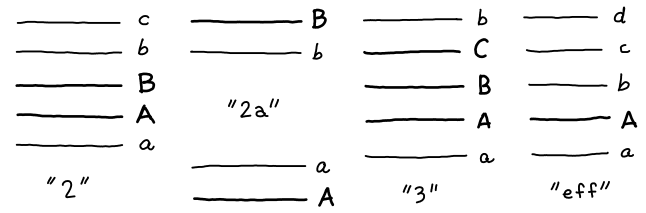
\includegraphics[width=30em]{modmisfinale}
	\caption{\label{fig:modmisfinale}
	Schema dei tipi di misura usati per il fit finale.
	Le linee orizzontali rappresentano le lastre di scintillatore;
	le lettere maiuscole indicano le lastre il cui conteggio in coincidenza
	viene usato per misurare il flusso (fa eccezione la configurazione ``eff''),
	le lettere minuscole indicano le lastre usate per misurare l'efficienza
	di quelle con le lettere maiuscole.}
\end{figure}

\subsubsection{Misure in coincidenza a 2}

\begin{figure}
	\centering
	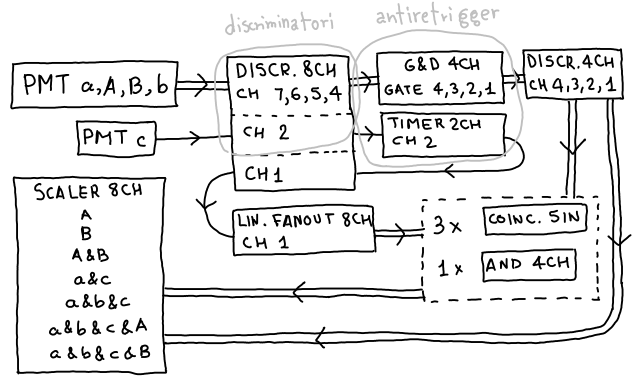
\includegraphics[width=30em]{circuitomisdue}
	\caption{\label{fig:circuitomisdue}
	Circuito per la misura in configurazione ``2''.
	Le linee di collegamento doppie rappresentano genericamente più di un cavo.
	I segnali dei PMT vanno ai discriminatori.
	Dopo i discriminatori ci sono i moduli \texttt{Gate\&Delay} e \texttt{Dual Timer}
	impostati su una durata di \SI{700}{ns} non retriggerabile;
	i segnali di questi passano da discriminatori <<secondo stadio>> (per distinguerli dagli altri)
	che riportano la durata dei segnali a circa~\SI{40}{ns}.}
\end{figure}

Usiamo il conteggio di due lastre (chiamate $A$ e $B$) in coincidenza per misurare il flusso
e tre lastre in coincidenza ($a$, $b$ e $c$) per misurare le efficienze di $A$ e $B$
(vedi configurazione ``2'' in \autoref{fig:modmisfinale}).
Usare solo due lastre in coincidenza ci permette di scegliere le lastre più vicine possibili nel nostro apparato
e quindi di avere l'accettanza geometrica maggiore possibile.
Usiamo altre tre lastre per l'efficienza anziché due in modo da non doverci preoccupare del rumore.
Nella maggior parte delle misure le lastre $A$ e $B$ sono comprese tra le lastre $a$, $b$ e $c$
in modo che la misura dell'efficienza dipenda trascurabilmente dalla distribuzione angolare.
Complessivamente quindi questa misura è ottimizzata per il flusso totale.

Il circuito è riportato in \autoref{fig:circuitomisdue}.
I circuiti delle altre configurazioni sono in sostanza uguali.
I dati sono riportati in \autoref{tab:data2}.
\marginpar{Nel cerchio di antiretrigger includere anche i discriminatori secondo stadio
per coerenza con i circuiti dell'ADC.}

\subsubsection{Misure in coincidenza a 2 con distribuzione angolare}

Questa configurazione (``2a'' in \autoref{fig:modmisfinale}) è simile alla precedente,
ma le lastre usate per misurare l'efficienza sono comprese tra quelle usate per misurare il flusso anziché esterne.
Questo ci permette di scegliere le lastre $A$ e $B$ il più lontane possibile
in modo da essere particolarmente sensibili alla densità verticale di raggi.
Le due lastre aggiuntive sono comunque disposte in modo da minimizzare
la dipendenza dall'accettanza della misura di efficienza.
Le lastre aggiuntive sono due ($a$ e $b$) anziché tre
perché usiamo anche $B$ per misurare l'efficienza di $A$ e viceversa.
I dati sono riportati in \autoref{tab:data2a}.

\subsubsection{Misure in coincidenza a 3}

In questa configurazione (``3'' in \autoref{fig:modmisfinale})
usiamo tre lastre ($A$, $B$ e $C$) in coincidenza per misurare il flusso
e due lastre ($a$ e $b$) esterne ad $A$, $B$ e $C$ per misurare l'efficienza di $A$, $B$ e $C$.
In questo modo non dobbiamo preoccuparci del rumore sulle lastre con cui misuriamo il flusso.
È interessante confrontare questa misura con una della configurazione ``2'' tale che $A_2=A_3$ e $B_2=C_3$.
\marginpar{Modo più chiaro (sintetitico) di dirlo?}
I dati sono riportati in \autoref{tab:data3}.

\subsubsection{Misure di efficienza con distribuzione angolare}

Questa configurazione (``eff'' in \autoref{fig:modmisfinale})
è abbastanza diversa dalle altre perché è ottimizzata per la distribuzione angolare anziché per il flusso.
Misuriamo l'efficienza di una lastra $A$ con varie coppie delle lastre $a$, $b$, $c$, $d$.
Imponendo che l'efficienza di $A$ sia la stessa e scegliendo in modo opportuno le coppie
si ottiene un forte vincolo sulla distribuzione angolare dei raggi.
Delle lastre minuscole almeno una è dal lato opposto di $A$ rispetto alle altre in modo
da avere almeno una misura di efficienza che non dipende dalla distribuzione angolare.
I dati sono riportati in \autoref{tab:dataeff}.

\subsection{Fit}

Eseguiamo un fit ai minimi quadrati sui dati della misura finale
per ricavare il flusso per unità di area orizzontale $\Phi$
(vedi \autoref{sec:teogeom} per la notazione) e la distribuzione angolare.
Per la distribuzione angolare prendiamo il modello $p(u) = (\alpha+1) u^\alpha$.
Oltre a $\Phi$ e $\alpha$ ci sono i nuisance parameters $\epsilon_i$
che sono le efficienze del PMA in ognuna delle misure di tipo ``eff''.
Per ogni misura di tipo ``2'', ``2a'' e ``3'' calcoliamo il flusso;
per ogni misura di tipo ``eff'' calcoliamo tre efficienze.
Il vettore $\mathbf r$ dei residui è dato dalla differenza dei flussi con il parametro $\Phi$
e dalla differenza delle triplette di efficienze con i parametri $\epsilon_i$ (uno per tripletta).
La forma quadratica da minimizzare è
\begin{equation*}
	X = \mathbf r^\top V^{-1} \mathbf r,
\end{equation*}
dove $V$ è la matrice di covarianza di $\mathbf r$.
La $V$ è calcolata con propagazione al primo ordine.
Nei calcoli sottraiamo le coincidenze casuali con la formula al primo ordine
dalle coincidenze a 2 e, quando i rate sono piuttosto alti, anche dalle coincidenze a~3.
Teniamo conto di tutte le correlazioni, con queste eccezioni:
\begin{itemize}
	\item Non tutte le accettanze possono essere calcolate con lo stesso pivot;
	il nostro codice non calcola la correlazione tra accettanze calcolate con pivot diversi
	ma un algoritmo sceglie i pivot in modo che la maggior parte delle correlazioni venga calcolata.
	L'incertezza del calcolo delle accettanze è comunque mantenuta più piccola delle altre.
	\item Nel calcolo delle efficienze per le misure ``eff'' e ``2a''
	non calcoliamo la correlazione tra i vari rapporti di conteggi;
	tuttavia stimiamo che sia piccola.
	Per le efficienze nelle misure ``2'' e ``3'' abbiamo calcolato
	che la correlazione tra i rapporti di conteggi è nulla
	(vedi \autoref{sec:vareff}).
\end{itemize}

\paragraph{Monte Carlo}

Poiché il calcolo delle accettanze è un Monte Carlo che dipende da $\alpha$,
dobbiamo fissare i campioni con cui eseguiamo il calcolo
in modo che $X$ sia effettivamente una funzione di $\alpha$.
Anche la distribuzione dei campioni dipende da $\alpha$,
quindi prima della minimizzazione estraiamo dei campioni uniformi
e poi nel fit applichiamo una statistica che dipende da $\alpha$ per ottenere la distribuzione.

\paragraph{Covarianza della stima}

Per stimare la matrice di covarianza della stima dei parametri
usiamo il metodo standard di invertire la matrice di curvatura (l'hessiana) di $X/2$.
Tuttavia $X$ non è derivabile con i metodi numerici standard rispetto ad $\alpha$ perché
il calcolo Monte Carlo è per sua natura discreto.
Allora calcoliamo la curvatura in questo modo:
\begin{description}
	\item[Termini diagonali]
		Calcoliamo $X/2$ in 10 punti al variare del parametro rispetto al quale dobbiamo derivare intorno al minimo,
		tenendo fissi gli altri nel minimo. I punti più lontani sono tali che 
		Su questi punti facciamo il fit di una parabola $\frac12a(x-x_0)^2+y_0$;
		il parametro $a$ è la curvatura.
	\item[Termini fuori diagonale]
		Siano $p$ e $q$ i due parametri rispetto a cui dobbiamo derivare;
		siano $a_p$ e $a_q$ le curvature già calcolate.
		Calcoliamo 10 punti intorno al minimo variando $(p,q)$ lungo la direzione $(1/\sqrt{a_p},1/\sqrt{a_q})$,
		siano $(\mathbf p,\mathbf q)$ questi punti.
		Fittiamo la parabola $\frac12a(x-x_0)^2+y_0$ dove $\mathbf x=\mathbf p\sqrt{a_p} + \mathbf q\sqrt{a_q}$.
		Sia $a_{pq}$ il risultato per $a$, allora la derivata incrociata è data da
		\begin{equation*}
			\frac{\partial^2}{\partial p\partial q} \frac X2 = (2a_{pq} - 1)\sqrt{a_p}\sqrt{a_q}.
		\end{equation*}
\end{description}

\paragraph{Incertezza geometrica}

L'incertezza geometrica (il cui calcolo è descritto in \autoref{sec:uncgeom})
è lenta da calcolare, quindi la calcoliamo in un punto iniziale e la teniamo fissa durante la minimizzazione.
Ripetiamo la minimizzazione due volte ricalcolando l'incertezza geometrica nel minimo trovato all'iterazione precedente;
i due minimi vengono praticamente identici quindi siamo sicuri della convergenza.

\paragraph{Prefit}

Poiché nel momento in cui abbiamo impostato e preso le misure
non avevamo ancora stabilito definitivamente se e come fare un fit,
abbiamo testato il fit solo su alcune misure, dette di prefit,
e eseguito il fit per dare il risultato finale sulle altre.
In questo modo evitiamo di introdurre un bias scegliendo come fare il fit in base al risultato.
Come misure di prefit abbiamo scelto quelle a statistica minore.
Per la configurazione ``3'', purtroppo, abbiamo una sola misura;
abbiamo deciso (rischiosamente) di non usarla nel prefit e aggiungerla solo nel fit finale.

%--------------------------- TABELLONE ------------------------------

% l'ambiente {landscape} gira la pagina in orizzontale quando la vedi a schermo e la lascia verticale quando stampi.
\begin{landscape}
	\begin{table}[p]
		\centering
		\small
		\begin{tabular}{llll|lrrrrrrr|ccccc|c}
			sogliaA & sogliaB & alimA & alimB & clock & A & B & A\&B & a\&c & a\&b\&c & a\&b\&c\&A & a\&b\&c\&B & PMA & PMB & PMa & PMb & PMc & prefit \\
			\hline\hline
			597 & 1014 & 1900 & 1900 & 1e5 & 7513 & 16958 & 1632 & 1140 & 1054 & 764 & 842 & 3 & 4 & 2 & 5 & 6 & 1                          \\
			597 & 1014 & 1900 & 1900 & 3e5 & 22504 & 50217 & 4923 & 3677 & 3405 & 2426 & 2748 & 3 & 4 & 2 & 5 & 6 & 1                       \\
			597 & 1014 & 2000 & 2000 & 1e5 & 23688 & 89514 & 2286 & 1200 & 1110 & 1005 & 1049 & 3 & 4 & 2 & 5 & 6 & 1                       \\
			597 & 1014 & 2000 & 2000 & 1e5 & 24057 & 85104 & 2317 & 1293 & 1207 & 1081 & 1115 & 3 & 4 & 2 & 5 & 6 & 1                       \\
			471 & 1014 & 2000 & 2000 & 1e5 & 85713 & 84140 & 2391 & 1241 & 1149 & 1044 & 1071 & 3 & 4 & 2 & 5 & 6 & 1                       \\
			398 & 628 & 2000 & 2000 & 1e5 & 336320 & 337053 & 2699 & 1238 & 1141 & 1042 & 1079 & 3 & 4 & 2 & 5 & 6 & 1                      \\
			398 & 628 & 2000 & 2000 & 1e5 & 347229 & 339499 & 2678 & 1272 & 1150 & 1054 & 1098 & 3 & 4 & 2 & 5 & 6 & 1                      \\
			398 & 628 & 2000 & 2000 & 1e6 & 3486673 & 3654718 & 26777 & 12175 & 11163 & 10307 & 10608 & 3 & 4 & 2 & 5 & 6 & 0               \\
			447 & 793 & 2000 & 2000 & 54413944 & 93555166 & 107266650 & 1370413 & 675409 & 620744 & 567583 & 586641 & 3 & 4 & 2 & 5 & 6 & 0 \\
			447 & 793 & 2000 & 2000 & 5428946 & 12407950 & 15049021 & 141548 & 67278 & 61960 & 56592 & 58785 & 3 & 4 & 2 & 5 & 6 & 0        \\
			\hline
			447 & 29.72 & 2000 & 2000 & 1e5 & 218729 & 116204 & 2074 & 1247 & 1136 & 1048 & 1098 & 3 & 5 & 2 & 4 & 6 & 1                       \\
			447 & 29.72 & 2000 & 2000 & 74832702 & 98917344 & 88277251 & 1550323 & 928983 & 847036 & 783834 & 826330 & 3 & 5 & 2 & 4 & 6 & 0   \\
			447 & 29.72 & 2000 & 2000 & 1e5 & 335083 & 204463 & 2061 & 1249 & 1120 & 1037 & 1095 & 3 & 5 & 2 & 4 & 6 & 1    \\   %   senza telo nero 
			76.5 & 29.72 & 2000 & 2000 & 1e5 & 4134344 & 187105 & 2838 & 1268 & 1159 & 1076 & 1100 & 3 & 5 & 2 & 4 & 6 & 1      \\   %  senza telo nero  
			30.73 & 29.72 & 2000 & 2000 & 1e5 & 4426281 & 186124 & 3000 & 1256 & 1117 & 1039 & 1068 & 3 & 5 & 2 & 4 & 6 & 0     \\  %  # senza telo nero
			\hline
			30.73 & 29.72 & 2000 & 2000 & 1e5 & 120570 & 97688 & 1867 & 522 & 480 & 458 & 463 & 2 & 5 & 1 & 4 & 6 & 1                             \\
			30.73 & 29.72 & 2000 & 2000 & 1e6 & 1206351 & 977575 & 19370 & 5387 & 4949 & 4749 & 4808 & 2 & 5 & 1 & 4 & 6 & 0                      \\
			\hline
			% forse le due prossime due misure avranno qualcosa che non va
			% -> confermo dal prefit che sono molto sballate anche supponendo che i raggi siano verticali
			% 307.3 & 297.2 & 2000 & 2000 & 1e5 & 121504 & 253216 & 1574 & 680 & 603 & 570 & 472 & 2 & 6 & 1 & 4 & 5 & 1
			% 307.3 & 1.517e3 & 2000 & 2000 & 1e5 & 122622 & 131362 & 1467 & 756 & 720 & 641 & 528 & 2 & 6 & 1 & 4 & 5 & 1
			30.73 & 151.7 & 2000 & 2000 & 1e6 & 1233265 & 1329361 & 14334 & 7256 & 6400 & 6056 & 4909 & 2 & 6 & 1 & 4 & 5 & 0                   \\
			30.73 & 151.7 & 2000 & 2000 & 1e5 & 122701 & 134106 & 1480 & 751 & 676 & 646 & 532 & 2 & 6 & 1 & 4 & 5 & 1                          \\
			30.73 & 29.73 & 2000 & 2000 & 1e5 & 122750 & 253274 & 1492 & 687 & 605 & 567 & 477 & 2 & 6 & 1 & 4 & 5 & 0                            \\
			\hline
			30.73 & 29.73 & 2000 & 2000 & 1e5 & 125673 & 111377 & 1971 & 538 & 493 & 466 & 482 & 2 & 5 & 1 & 4 & 6 & 1                            \\
			30.73 & 29.73 & 2000 & 2000 & 12840754 & 13958014 & 14572786 & 255165 & 68855 & 63402 & 60630 & 62120 & 2 & 5 & 1 & 4 & 6 & 0         
		\end{tabular}
		\caption{\label{tab:data2}
		Dati per la configurazione ``2'' della misura finale.
		I dati sono riportati in ordine cronologico di acquisizione.
		Le colonne <<soglia\dots>> riportano la soglia del discriminatore in millivolt.
		Le colonne <<alim\dots>> riportano la tensione nominale di alimentazione dei PMT in volt.
		La colonna <<clock>> riporta il conteggio del \texttt{clock} del contatore,
		quindi il tempo di acquisizione in millesimi di secondo.
		Le colonne successive a <<clock>> sono i conteggi; le <<\&>> indicano le coincidenze.
		Le colonne <<PM\dots>> indicano a quali PM corrispondono le etichette $A$, $B$, $a$, $b$, $c$;
		le linee orizzontali nella tabella demarcano il cambiamento degli assegnamenti.
		La colonna <<prefit>> indica se i dati vengono utilizzati nel fit preliminare (1) o nel fit finale (0).
		Le durate dei discriminatori secondo stadio (vedi circuito in \autoref{fig:circuitomisdue})
		sono \SI{38\pm2}{ns} per $A$ e \SI{37\pm2}{ns} per $B$.
		Il secondo stadio di $a$, $b$ e $c$ è a circa \SI{40}{ns}.}
	\end{table}
\end{landscape}

\begin{table}[p]
	% \centering
	\small
	\hspace{-5em}
	\begin{tabular}{ll|lrrrrrrr|c}
		sogliaA & sogliaB & clock & A & B & A\&B & a\&b & a\&b\&B & a\&b\&A & a\&b\&A\&B & prefit \\
		\hline
		30.73 & 29.73 & 1e5 & 1008979 & 270259 & 920 & 1763 & 1224 & 702 & 555  & 1               \\
		30.73 & 29.73 & 1e6 & 9995686 & 2690915 & 9059 & 17919 & 12177 & 6977 & 5346 & 0          \\
		146.8 & 183.2 & 1e5 & 98858 & 92615 & 601 & 1859 & 1221 & 688 & 509  & 1                    \\
		146.8 & 183.2 & 1e6 & 988694 & 926201 & 5550 & 17807 & 11758 & 6195 & 4645 & 0              \\
		128.7 & 96.4 & 1e5 & 197923 & 205786 & 634 & 1708 & 1160 & 615 & 487  & 1            \\
		128.7 & 96.4 & 1e6 & 1996164 & 2070802 & 6443 & 17532 & 11819 & 6397 & 4922 & 0      
	\end{tabular}
	\caption{\label{tab:data2a}
	Dati per la misura finale in configurazione ``2a''.
	La notazione è la stessa della \autoref{tab:data2}.
	Tutte le misure sono state fatte con $A$ = PM1, $B$ = PM6, $a$ = PM2, $b$ = PM5.
	L'alimentazione di $A$ e $B$ è \SI{2000}V.
	Le durate del secondo stadio sono le stesse della configurazione ``2''.}
\end{table}

\begin{table}[p]
	\small
	\hspace{-9em}
	\begin{tabular}{lll|rrrrrrrr|c}
		sogliaA & sogliaB & sogliaC & clock & C & B & A\&B\&C & a\&b & a\&b\&C & a\&b\&B & a\&b\&A & prefit \\
		\hline
		30.71 & 29.71 & 20.71 & 53093476 & 62962492 & 723662210 & 1073466 & 668411 & 617769 & 607441 & 591279 & 0
	\end{tabular}
	\caption{\label{tab:data3}
	Dati per la misura finale in configurazione ``3''.
	La notazione è la stessa della \autoref{tab:data2}.
	Le tensioni di alimentazione di $A$ e $B$ sono \SI{2000}V.
	Le etichette sono $A$ = PM3, $B$ = PM4, $C$ = PM5, $a$ = PM2, $b$ = PM6.
	Le durate del secondo stadio per $A$ e $B$ sono le stesse della configurazione ``2''.
	Il secondo stadio di $a$, $b$ e $C$ è \SI{35\pm1}{ns}.
	Sono stati misurati separatamente i tassi di $A$, $a$ e $b$:
	su un clock di 1e5, i conteggi sono $C_A=4243753$, $C_a=86130$, $C_b=31799$.}
\end{table}

\begin{table}[p]
	\small
	\hspace{-10.5em}
	\begin{tabular}{l|rrrrrrrr|ccccc|c}
		sogliaA & clock & A &a\&b & a\&b\&A & b\&c & b\&c\&A & b\&d & b\&d\&A & PMA & PMa & PMb & PMc & PMd & prefit \\
		\hline\hline
		221.6 & 1e5   & 2862828 & 1989 & 1791 & 2630 & 1830 & 1908 & 1402 & 3 & 2 & 4 & 5 & 6 & 1           \\
		221.6 & 1e6   & 29620183 & 19040 & 17372 & 26445 & 18041 & 18864 & 13703 & 3 & 2 & 4 & 5 & 6 & 0     \\
		511 & 1e5 & 120032 & 1975 & 1782 & 2684 & 1804 & 1888 & 1362 & 3 & 2 & 4 & 5 & 6 & 1         \\
		30.65 & 1e5  & 4464209 & 1957 & 1790 & 2641 & 1833 & 1926 & 1421 & 3 & 2 & 4 & 5 & 6 & 1          \\
		\hline
		30.65 & 1e5  & 122838 & 965 & 922 & 2500 & 1847 & 1938 & 1443 & 2 & 1 & 3 & 4 & 5 & 1            \\
		30.65 & 1e6  & 1239854 & 9576 & 9163 & 24663 & 18227 & 19352 & 14530 & 2 & 1 & 3 & 4 & 5 & 0      \\
		146.0 & 1e5   & 104482 & 955 & 903 & 2465 & 1773 & 1961 & 1443 & 2 & 1 & 3 & 4 & 5 & 1             \\
		\hline
		146.0 & 1e5   & 50512 & 943 & 901 & 2465 & 1802 & 1454 & 1088 & 2 & 1 & 3 & 4 & 6 & 0             
	\end{tabular}
	\caption{\label{tab:dataeff}
	Dati per la misura finale in configurazione ``eff''.
	La notazione è la stessa della \autoref{tab:data2}.
	Le alimentazioni sono
	$V_1=\SI{2000}V$, $V_2=\SI{2000}V$, $V_3=\SI{1900}V$, $V_4=\SI{1950}V$, $V_5=\SI{2000}V$, $V_6=\SI{2000}V$,
	ad eccezione di $A$ che è sempre a \SI{2000}V.
	I~rate di $a$, $b$, $c$, $d$ sono sempre circa \SI{500}{s^{-1}}.}
\end{table}


\begin{thebibliography}{99} % Bibliography

\bibitem[1] {1}
Laurie M. Unger, D. K. Trubey, Specific gamma-ray dose constants for nuclides important to dosimetry and radiological assessment, ORNL/RSIC-45/RI, \emph{Oak Ridge National Laboratory} (1982).

\bibitem[2] {2}
S.Y.F. Chu, L.P. Ekström, R.B. Firestone, The Lund/LBNL Nuclear Data Search Version 2.0, \emph{Berkeley National Laboratory} (1999).

\bibitem[3]{3}
M.J. Berger, J.S. Coursey, M.A. Zucker, J. Chang, Stopping-power \& range tables for electrons, protons, and helium ions, \emph{National Institute of Standards and Technology} (2017).

\bibitem[4]{4}
K.A. Olive et al., Passage of particles through matter, (PDG), Chin. Phys. C38, 090001 (2014).

\bibitem[5]{5}
M.J. Berger, J.H. Hubbell, S.M. Seltzer, J. Chang, J.S. Coursey, R. Sukumar, D.S. Zucker, and K. Olsen, XCOM: Photon Cross Sections Database XCOM, \emph{National Institute of Standards and Technology} (2010).

\bibitem[6]{6}
G.F. Knoll, Radiation Detection and Measurement- 3rd edition (Capitolo 10), \emph{Wiley} (1999).

\bibitem[7]{7}
P. M. Bergstrom Jr, Compton scattering of photons from electrons bound in light elements, \emph{Argonne National Laboratory} (1994).

\bibitem[8]{8}
P.M. Bergstrom Jr, R.H. Pratt, An overview of the theories used in Compton scattering calculation, \emph{Radiat. Phys. Chem.} Vol. 50, No. 1, pp. 3-29 (1997).

\end{thebibliography}


\end{document}